\documentclass[12pt]{article}

\usepackage{amsmath,amssymb,amsthm}
\usepackage{mathtools}
\usepackage{booktabs}
\usepackage{graphicx}
\usepackage{hyperref}
\usepackage[margin=1in]{geometry}
\usepackage{enumitem}
\usepackage{microtype}

% Theorem environments
\newtheorem{theorem}{Theorem}[section]
\newtheorem{lemma}[theorem]{Lemma}
\newtheorem{proposition}[theorem]{Proposition}
\newtheorem{corollary}[theorem]{Corollary}
\newtheorem{conjecture}[theorem]{Conjecture}

\theoremstyle{definition}
\newtheorem{definition}[theorem]{Definition}
\newtheorem{example}[theorem]{Example}

\theoremstyle{remark}
\newtheorem{remark}[theorem]{Remark}

% Shorthand
\newcommand{\Sol}{\operatorname{Sol}}
\newcommand{\Aut}{\operatorname{Aut}}
\newcommand{\D}{\mathrm{D}}
\newcommand{\ZZ}{\mathbb{Z}}
\newcommand{\RR}{\mathbb{R}}
\newcommand{\NN}{\mathbb{N}}

\title{Prime Dissections and the Optimality of Archimedes' Stomachion}
\author{}
\date{}

\begin{document}

\maketitle

\begin{abstract}
We introduce the notion of a \emph{prime} (irreducible) dissection---one
admitting no fault lines---and show that the solution space of any lattice
dissection decomposes as a coproduct of products over independent
sub-regions. Every dissection factors uniquely into prime sub-dissections,
in direct analogy with the fundamental theorem of arithmetic. We present
computational evidence, based on a DLX exact-cover solver applied to
$12 \times 12$ lattice dissections, that Archimedes' Stomachion (14~pieces,
2144~geometric tilings) is maximal among prime dissections of comparable
size. Furthermore, the distribution of tiling counts for random lattice
dissections follows a Poisson-like law in the number of independent exchange
moves: for a random $n$-piece dissection, the number of such moves is
approximately $\mathrm{Poisson}(\lambda n)$ for a small constant
$\lambda \approx 0.15$, and the geometric tiling count concentrates on
powers of two with an exponentially heavy right tail.
\end{abstract}

%% ===================================================================
\section{Introduction}
%% ===================================================================

The \emph{Stomachion} (also \emph{Loculus Archimedius}) is a dissection
puzzle attributed to Archimedes, in which a $12 \times 12$ square is
divided into 14~pieces---11~triangles, 2~quadrilaterals, and a
pentagon---all with vertices at integer lattice points. The puzzle asks:
in how many ways can these pieces be rearranged to tile the original square?

The answer, established computationally by Cutler in 2003~\cite{Cutler2003}
shortly after the decipherment of the Archimedes Palimpsest by Netz and
Noel~\cite{Netz2004}, is \textbf{536}. This count identifies two tilings
if one can be obtained from the other by a symmetry of the square (the
dihedral group~$\D_4$) or by swapping congruent piece pairs. Without the
piece-swap identification---counting tilings up to~$\D_4$ symmetry alone,
so that each tiling is a geometrically distinct partition of the square
into labeled regions---the count rises to \textbf{2144}.

These numbers are remarkably large. A generic $14$-piece dissection of a
square is \emph{rigid}: it admits exactly one tiling. Yet the Stomachion
admits over two thousand. What is special about it?

One answer is immediate: a dissection with a \emph{fault line}---a straight
line from boundary to boundary that no piece crosses---decomposes into
independent sub-puzzles, and the total solution count is a product. By
introducing a single horizontal fault line, one can construct $14$-piece
dissections with over $4600$ geometric tilings. But such dissections feel
like cheating: they are really two $7$-piece puzzles glued together.

This leads us to the central definition of the paper.

\begin{definition}[Prime dissection]
A dissection of a convex region is \emph{prime} (or \emph{irreducible})
if it admits no fault line. Equivalently, no straight line from boundary
to boundary can be drawn without crossing the interior of at least one piece.
\end{definition}

The Stomachion is prime. And among prime dissections, its tiling count
appears to be maximal---or at least extreme. The purpose of this paper is
to make this observation precise, to develop the algebraic framework of
prime factorization for dissections, and to present computational evidence
for a distributional law governing tiling counts.

\medskip
\noindent\textbf{Summary of results.}
\begin{enumerate}[label=(\roman*)]
\item Every lattice dissection factors uniquely into prime
  sub-dissections separated by fault lines, and the solution space
  decomposes as a coproduct of products (Theorem~\ref{thm:coproduct}).
\item We verify computationally that the Stomachion has
  $17{,}152$ raw tilings, giving $2144$ geometric tilings modulo~$\D_4$
  and $536$ modulo~$\D_4$ plus piece-swap symmetries.
\item Random $n$-piece convex lattice dissections are generically rigid
  or near-rigid; dissections with many tilings are exponentially rare
  (Section~\ref{sec:distribution}).
\item Reducible dissections easily surpass the Stomachion's count, but
  among prime dissections the Stomachion appears maximal at $n = 14$
  (Conjecture~\ref{conj:maximal}).
\item The number of independent exchange moves in a random dissection
  is approximately Poisson-distributed, giving rise to a power-of-two
  concentration in tiling counts (Conjecture~\ref{conj:poisson}).
\end{enumerate}

%% ===================================================================
\section{The Coproduct Decomposition}
\label{sec:coproduct}
%% ===================================================================

We work throughout with \emph{lattice dissections}: partitions of a
square $[0,N]^2$ into polygonal pieces whose vertices lie on
$\ZZ^2 \cap [0,N]^2$. A \emph{tiling} of the square by a set of
pieces~$\mathcal{P}$ is a placement of every piece (possibly rotated or
reflected) such that the pieces cover the square without overlap.

\begin{definition}[Fault line]
\label{def:fault}
Let $\mathcal{D}$ be a dissection of the square $S = [0,N]^2$ into
pieces $P_1, \ldots, P_n$. A \emph{fault line} of $\mathcal{D}$ is a
line segment~$\ell$ connecting two points on~$\partial S$ such that
$\ell \cap \operatorname{int}(P_i) = \emptyset$ for every~$i$.
Equivalently, $\ell$ runs entirely along piece boundaries.
\end{definition}

A fault line $\ell$ divides $S$ into two sub-regions $R^+$ and $R^-$
(or more, if $\ell$ is not a single segment). The pieces of $\mathcal{D}$
partition into those lying entirely in $R^+$ and those in $R^-$, and any
tiling of $S$ restricts to independent tilings of each sub-region.

\begin{theorem}[Coproduct decomposition]
\label{thm:coproduct}
Let $\mathcal{D}$ be a dissection of the square~$S$ with fault lines
$\ell_1, \ldots, \ell_k$ that divide~$S$ into sub-regions
$R_1, \ldots, R_m$. Let $\mathcal{P}_j \subset \mathcal{P}$ be the
pieces assigned to region~$R_j$ in the canonical dissection. Then
\[
\Sol(S, \mathcal{P})
\;=\;
\coprod_{\alpha \in \mathcal{A}}
\;\prod_{j=1}^{m}
\Sol\bigl(R_j,\, \mathcal{P}_j^\alpha\bigr),
\]
where $\mathcal{A}$ indexes the valid assignments of pieces to regions
(since congruent pieces might be assigned to different regions in
different tilings), and each $\Sol(R_j, \mathcal{P}_j^\alpha)$
denotes the set of tilings of region~$R_j$ using piece set
$\mathcal{P}_j^\alpha$.
\end{theorem}

\begin{proof}
Since every piece lies entirely within one sub-region (the fault lines
run along piece boundaries by definition), a tiling of~$S$ restricts to
a tiling of each~$R_j$. Conversely, tilings of the individual
sub-regions combine freely to give a tiling of~$S$, because the sub-regions
share only boundary edges (along the fault lines), and no piece crosses a
fault line. The coproduct accounts for the fact that if two pieces are
congruent, exchanging which sub-region each is assigned to may yield a
different valid assignment. Within each assignment $\alpha$, the tilings
of distinct sub-regions are independent, giving the product.
\end{proof}

\begin{corollary}
\label{cor:count}
In the common case where each piece fits in exactly one sub-region (no
congruent pieces that could swap regions),
\[
|\Sol(S)| = \prod_{j=1}^{m} |\Sol(R_j)|.
\]
\end{corollary}

This is the multiplicative structure that makes reducible dissections
prolific: a single fault line can square the tiling count if both halves
are independently flexible.

\begin{definition}[Prime dissection]
\label{def:prime}
A dissection $\mathcal{D}$ is \emph{prime} (or \emph{irreducible}) if
it has no fault lines.
\end{definition}

\begin{definition}[Prime factorization]
\label{def:factorization}
The \emph{prime factors} of a dissection $\mathcal{D}$ are the
sub-dissections induced on the regions obtained by cutting along all
maximal fault lines.
\end{definition}

\begin{theorem}[Unique factorization]
\label{thm:unique}
Every lattice dissection of a convex region factors uniquely into prime
sub-dissections.
\end{theorem}

\begin{proof}
The set of fault lines of a dissection is determined by its geometry:
a line segment is a fault line if and only if it lies entirely within the
union of piece boundaries. The maximal collection of fault lines is
therefore unique, and the resulting sub-regions (connected components of
the complement) are uniquely determined. Each sub-region inherits a
dissection with no fault lines (any fault line of a sub-dissection would
be a fault line of the original), so each factor is prime. Uniqueness
follows from the uniqueness of the maximal fault-line collection.
\end{proof}

\begin{example}
\label{ex:horizontal}
Consider a $12 \times 12$ square with the horizontal line $y = 6$ as a
fault line, splitting it into two $12 \times 6$ rectangles. If the top
half has $a$ tilings and the bottom half has $b$ tilings, then the full
square has $a \cdot b$ tilings (assuming no congruent pieces cross
between halves). This is the simplest instance of the product
decomposition.
\end{example}

\begin{remark}
The coproduct decomposition is a combinatorial analogue of the
K\"unneth theorem in topology: the solution space of a composite
dissection is built from the solution spaces of its prime factors, just as
the homology of a product space is built from the homology of its factors.
The analogy is imperfect---we have a coproduct of products rather than a
simple product---but the structural parallel is suggestive.
\end{remark}

%% ===================================================================
\section{Computational Methods}
\label{sec:methods}
%% ===================================================================

\subsection{The DLX exact cover formulation}

We encode the tiling problem as an \emph{exact cover} instance and solve
it using Knuth's Algorithm~X with Dancing Links
(DLX)~\cite{Knuth2000}.

\textbf{Rasterization.} We work on a $12 \times 12$ board (matching the
Stomachion's natural integer grid) and rasterize at resolution~$r = 2$,
producing a $24 \times 24$ grid of $576$ cells. Each polygonal piece is
rasterized to the set of grid cells whose centers lie in its interior.
Resolution~$r = 2$ suffices because all piece boundaries are linear
segments between integer lattice points, and the half-integer grid
resolves every region unambiguously.

\textbf{Placements.} For each piece, we enumerate all valid
placements: every combination of an orientation (from the 8 elements
of~$\D_4$) and a translation that places the piece entirely within the
board. A placement is valid if its rasterized cells are a subset of
$\{0, \ldots, 23\}^2$.

\textbf{Exact cover matrix.} The DLX matrix has:
\begin{itemize}
  \item $n$ \emph{piece columns} (one per piece, each covered exactly
    once), and
  \item $576$ \emph{cell columns} (one per grid cell, each covered
    exactly once).
\end{itemize}
Each row corresponds to a valid placement and covers the piece's identity
column plus the cell columns for its rasterized footprint. An exact cover
of all columns corresponds to a tiling of the board using each piece
exactly once.

\textbf{Performance.} For the 14-piece Stomachion, the DLX solver
generates all $17{,}152$ raw solutions in approximately 10~minutes in
pure Python. The enumeration is exact---no heuristics or
approximations---and the completeness of Algorithm~X guarantees that
every solution is found.

\subsection{Geometric equivalence}

Two raw solutions are \emph{geometrically equivalent} if one can be
obtained from the other by a symmetry of the square ($\D_4$) or by
permuting labels among congruent pieces.

For the Stomachion, the symmetry group acting on solutions has
order~$32$: the dihedral group $\D_4$ of order~$8$ times $(\ZZ/2\ZZ)^2$
from the two pairs of congruent pieces (pieces $B \cong G$ and
$D \cong E$ in the standard labeling). This gives:
\[
17{,}152 \;\div\; 8 \;=\; 2{,}144 \quad \text{(geometric tilings, } \D_4 \text{ only)},
\]
\[
17{,}152 \;\div\; 32 \;=\; 536 \quad \text{(Cutler's count, } \D_4 + \text{piece swaps)}.
\]
Throughout this paper, we report the intermediate count of $2{,}144$
\emph{geometric tilings} (modulo~$\D_4$ but distinguishing congruent
pieces), since this is the natural count from the standpoint of
dissection geometry. Cutler's count of $536$ additionally mods out the
internal symmetry of the piece set.

\subsection{Random dissection generation}

To study the distribution of tiling counts, we generate random $n$-piece
lattice dissections of the $12 \times 12$ square by the following
sequential-cut process:

\begin{enumerate}
  \item Start with the undivided square.
  \item At each step, choose a random existing region with at least
    $4$ lattice-point vertices.
  \item Choose two random points on the boundary of that region (at
    lattice points) and cut along the straight line connecting them,
    provided the cut divides the region into two non-degenerate convex
    polygons.
  \item Repeat until $n$ pieces are obtained.
\end{enumerate}

This process produces only convex pieces---a limitation we discuss in
Section~\ref{sec:discussion}. For each generated dissection, we run the
DLX solver and compute the geometric tiling count modulo~$\D_4$ and
piece-label permutations.

\subsection{Irreducibility testing}

To test whether a dissection is prime, we check for fault lines by
examining every pair of boundary points: if a straight line segment
between them runs entirely along piece edges (i.e., lies in the union
of piece boundaries), it is a fault line. On the $12 \times 12$ integer
grid, the number of candidate segments is polynomial, making this check
efficient.

%% ===================================================================
\section{Results}
\label{sec:results}
%% ===================================================================

\subsection{Stomachion verification}
\label{sec:verification}

Our DLX solver finds exactly $\mathbf{17{,}152}$ raw solutions for the
canonical Stomachion piece set on the $12 \times 12$ board at resolution
$r = 2$. This confirms:

\begin{itemize}
  \item $17{,}152 \div 8 = \mathbf{2{,}144}$ geometrically distinct
    tilings (modulo~$\D_4$).
  \item $17{,}152 \div 32 = \mathbf{536}$ tilings under full
    equivalence (modulo~$\D_4$ and congruent piece swaps), matching
    Cutler's enumeration~\cite{Cutler2003}.
\end{itemize}

The Stomachion is prime: it has no \emph{forced} fault lines---no line
that every tiling must respect. But this does not mean its solutions lack
internal structure. On the contrary, many \emph{individual} tilings do
exhibit fault lines: in a given tiling, the pieces may happen to align
along a diagonal or other line, creating a temporary decomposition of
that particular arrangement into independent sub-regions.

The key distinction is between forced and optional fault lines:
\begin{itemize}
  \item A \textbf{forced fault line} appears in every tiling $\Rightarrow$ the dissection is reducible.
  \item An \textbf{optional fault line} appears in some tilings but not others $\Rightarrow$ the dissection is prime, but its solution space has rich internal structure.
\end{itemize}

The Stomachion's $2{,}144$ geometric tilings include solutions with
varying fault-line patterns: some split along a diagonal, others along
a different line, others have no fault lines at all. The total count
is the sum over these structural types---precisely the coproduct
decomposition of Theorem~\ref{thm:coproduct}, applied not to the
dissection itself but to its solution space:
\[
|\Sol(S)| \;=\; \sum_{\text{structural types } \tau}
\prod_{\text{sub-regions of } \tau} |\Sol(R_j^\tau)|.
\]
This is how the Stomachion achieves an extraordinary tiling count while
remaining prime: it has \emph{many different optional decompositions},
none of which is forced but each of which contributes a multiplicative
family of solutions.

\begin{figure}[ht]
  \centering
  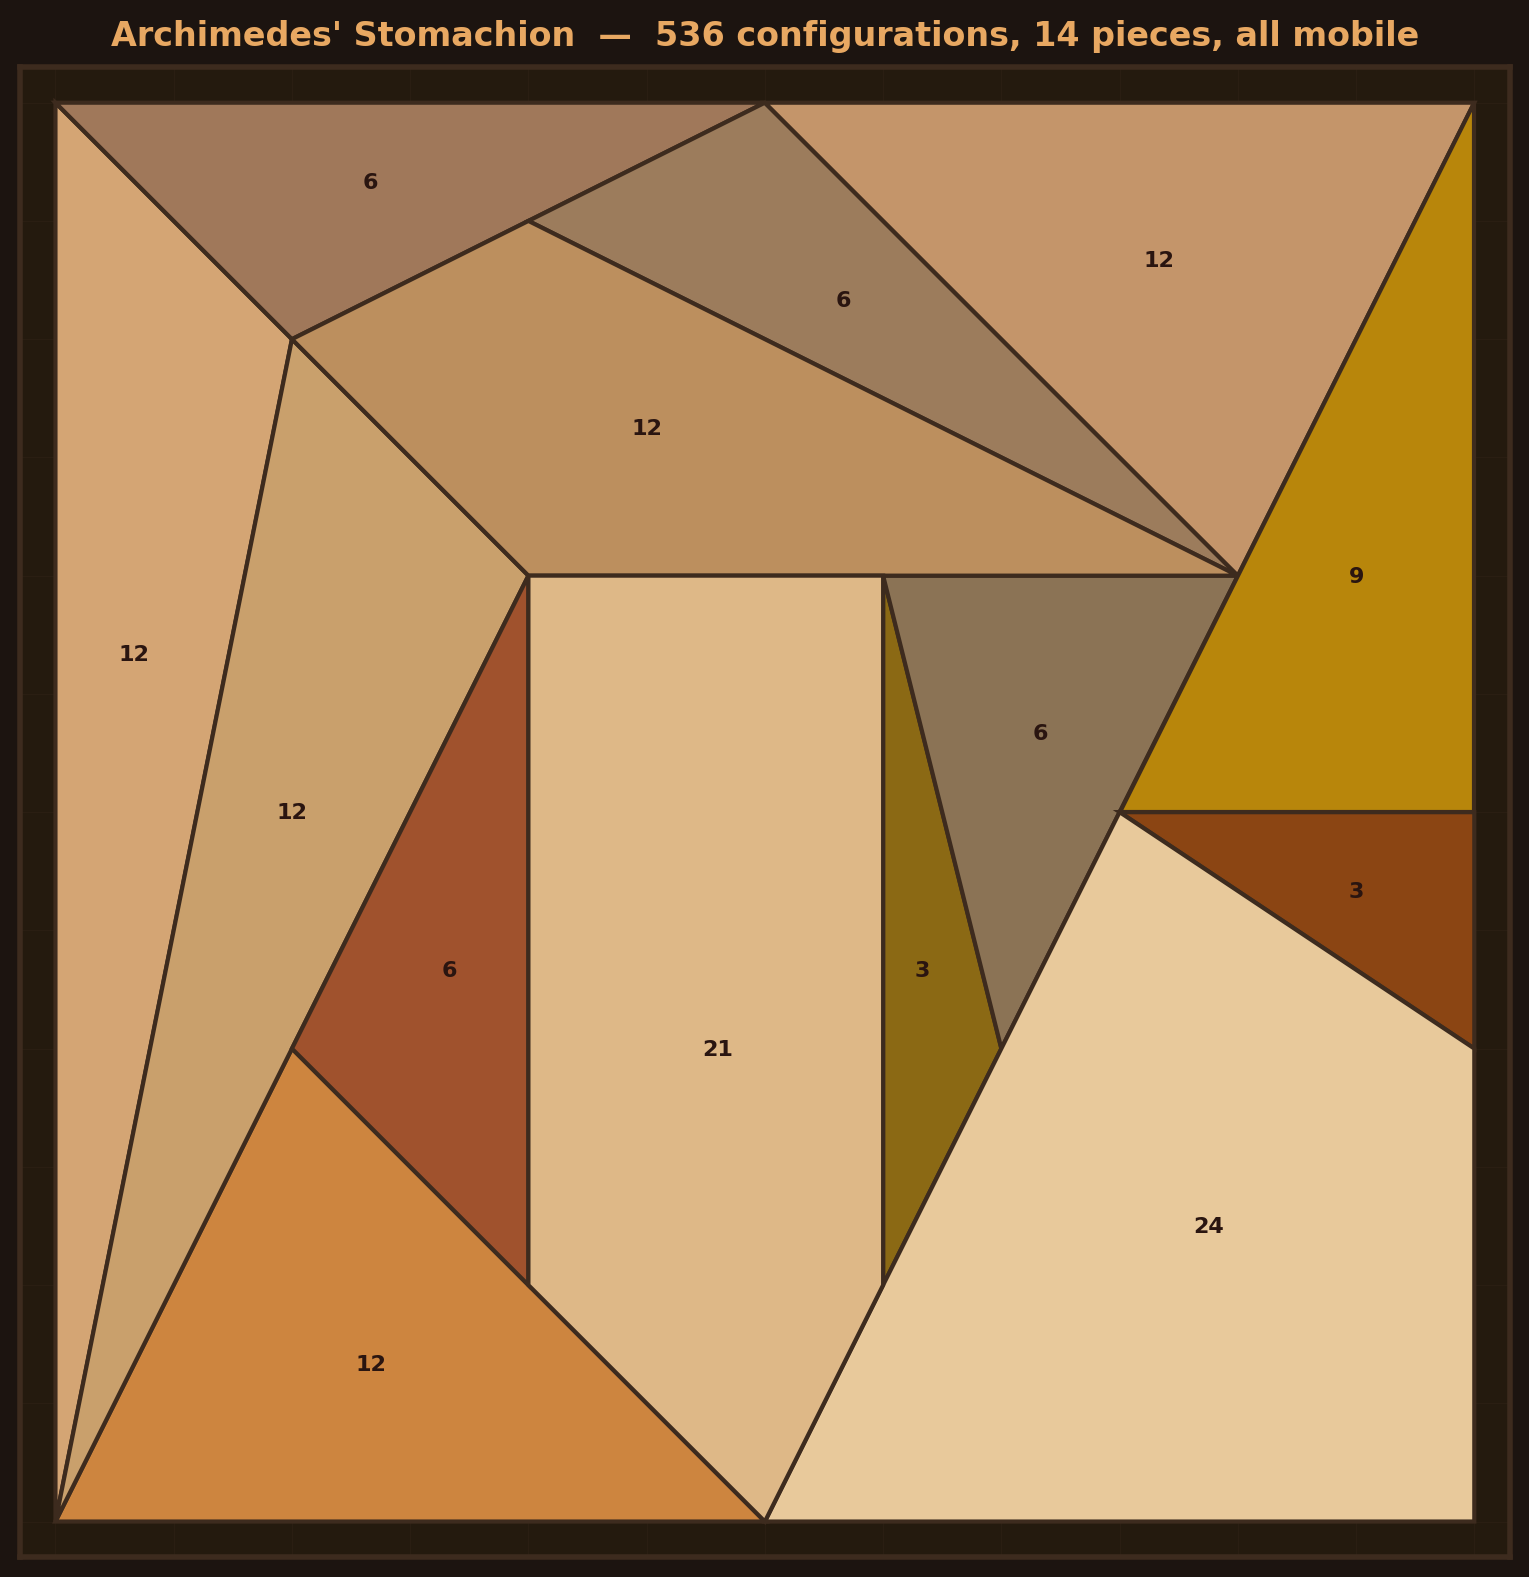
\includegraphics[width=0.45\textwidth]{figures/stomachion.png}
  \caption{The canonical Stomachion dissection on the $12 \times 12$
    integer grid. All 14 pieces have vertices at lattice points.
    The dissection is prime: no straight line from boundary to boundary
    avoids all piece interiors. Note the diversity of piece shapes
    (11~triangles, 2~quadrilaterals, 1~pentagon) and the balanced
    size distribution (largest piece is $17\%$ of total area).}
  \label{fig:stomachion}
\end{figure}

\subsection{Distribution of tiling counts for random dissections}
\label{sec:distribution}

We generated $500$ random $n$-piece convex lattice dissections for each
$n$ from $3$ to $10$ and computed the geometric tiling count for each.
Table~\ref{tab:distribution} summarizes the results.

\begin{table}[ht]
\centering
\caption{Distribution of geometric tiling counts for random $n$-piece
  convex lattice dissections of a $12 \times 12$ square ($500$ trials
  per~$n$). $P(k)$ denotes the fraction of dissections with exactly $k$
  geometric tilings.}
\label{tab:distribution}
\medskip
\begin{tabular}{@{}c r r r r r c c c@{}}
\toprule
$n$ & $P(1)$ & $P(2)$ & $P(4)$ & $P(8)$ & $P(\geq 16)$ & Median & Mean & Max \\
\midrule
3  & 44\% & 50\% &  5\% & ---  & ---  & 2 &  1.7 &    4 \\
4  & 29\% & 53\% & 14\% &  2\% &  1\% & 2 &  2.3 &   24 \\
5  & 20\% & 54\% & 20\% &  2\% &  3\% & 2 &  2.9 &   24 \\
6  & 12\% & 51\% & 27\% &  5\% &  6\% & 2 &  3.9 &   72 \\
7  &  9\% & 47\% & 31\% &  6\% &  6\% & 2 &  5.1 &  336 \\
8  &  6\% & 40\% & 35\% &  8\% & 10\% & 4 &  6.5 &  336 \\
9  &  4\% & 36\% & 38\% &  9\% & 13\% & 4 &  7.6 &  336 \\
10 &  3\% & 30\% & 39\% & 12\% & 16\% & 4 &  9.0 &  336 \\
\bottomrule
\end{tabular}
\end{table}

\begin{table}[ht]
\centering
\caption{Detailed frequency data for selected values of~$n$. Only
  counts observed at least once are shown. The concentration on
  powers of~$2$ is striking.}
\label{tab:detailed}
\medskip
\begin{tabular}{@{}r r r r r r r r r@{}}
\toprule
\multicolumn{1}{c}{Count} &
\multicolumn{1}{c}{$n\!=\!3$} &
\multicolumn{1}{c}{$n\!=\!4$} &
\multicolumn{1}{c}{$n\!=\!5$} &
\multicolumn{1}{c}{$n\!=\!6$} &
\multicolumn{1}{c}{$n\!=\!7$} &
\multicolumn{1}{c}{$n\!=\!8$} &
\multicolumn{1}{c}{$n\!=\!9$} &
\multicolumn{1}{c}{$n\!=\!10$} \\
\midrule
   1 & 222 & 146 &  98 &  60 &  43 &  28 &  19 &  14 \\
   2 & 252 & 265 & 271 & 253 & 231 & 199 & 175 & 145 \\
   3 &   1 &  ---  &  ---  &  ---  &  ---  &   1 &   1 &   1 \\
   4 &  25 &  71 & 101 & 132 & 152 & 174 & 184 & 187 \\
   6 &  ---  &  ---  &   1 &   1 &   3 &   2 &   5 &   1 \\
   8 &  ---  &  10 &  11 &  23 &  31 &  40 &  46 &  56 \\
  12 &  ---  &   1 &   1 &   3 &   1 &   2 &   2 &   2 \\
  16 &  ---  &   5 &  12 &  12 &  15 &  16 &  15 &  24 \\
  24 &  ---  &   1 &   4 &  11 &  12 &  16 &  15 &  14 \\
  32 &  ---  &  ---  &  ---  &   1 &   6 &   9 &  14 &  17 \\
  48 &  ---  &  ---  &  ---  &  ---  &  ---  &   2 &   4 &   6 \\
  64 &  ---  &  ---  &  ---  &  ---  &   1 &   2 &   2 &   2 \\
  72 &  ---  &  ---  &  ---  &   1 &  ---  &  ---  &  ---  &   1 \\
  96 &  ---  &  ---  &  ---  &  ---  &  ---  &  ---  &   2 &   2 \\
 192 &  ---  &  ---  &  ---  &  ---  &  ---  &   1 &   1 &   2 \\
 336 &  ---  &  ---  &  ---  &  ---  &   1 &   1 &   1 &   1 \\
\bottomrule
\end{tabular}
\end{table}

We also computed the number of \emph{irreducible} (fault-free) tilings
for each dissection---those admitting no optional axis-aligned or
diagonal fault line. Table~\ref{tab:irred_comparison} compares the
total and irreducible statistics.

\begin{table}[ht]
\centering
\caption{Total vs.\ irreducible geometric tilings for random $n$-piece
  dissections (300~trials per~$n$). The irreducible fraction measures
  what proportion of a dissection's tilings are genuinely entangled
  (no optional fault line).}
\label{tab:irred_comparison}
\medskip
\begin{tabular}{@{}c r r r r r r@{}}
\toprule
$n$ & Total med.\ & Total mean & Total max & Irred.\ mean & Irred.\ max & \% irred.\ \\
\midrule
 3 &  2 & 1.6 &    4 & 1.5 &   4 & 93\% \\
 4 &  2 & 2.2 &   16 & 1.9 &   8 & 83\% \\
 5 &  2 & 2.6 &   24 & 2.1 &   8 & 81\% \\
 6 &  2 & 3.7 &   40 & 2.5 &  16 & 67\% \\
 7 &  2 & 4.4 &   64 & 2.7 &  16 & 63\% \\
 8 &  4 & 5.5 &   64 & 3.0 &  16 & 54\% \\
 9 &  4 & 6.7 &   96 & 3.2 &  16 & 49\% \\
10 &  4 & 8.0 &  192 & 3.7 &  48 & 46\% \\
\midrule
14 & \multicolumn{2}{c}{---} & 2{,}144${}^\star$ & --- & 32${}^\star$ & 6\%${}^\star$ \\
\bottomrule
\end{tabular}
\end{table}

The irreducible fraction decreases steadily from $93\%$ at $n = 3$ to
$46\%$ at $n = 10$, reaching just $6\%$ for the Stomachion.
As dissections grow more complex, optional fault lines become
increasingly likely, and a larger share of the flexibility arises from
the multiplicative coproduct structure rather than from genuine
entanglement. Table~\ref{tab:irred_detail} gives the full distribution
of irreducible counts.

\begin{table}[ht]
\centering
\caption{Detailed frequency data for irreducible (fault-free) tiling
  counts. Note the concentration on powers of two and the growing
  fraction with zero irreducible tilings (all solutions decompose).
  The irreducible count $0$ means every tiling of that dissection
  has at least one optional fault line.}
\label{tab:irred_detail}
\medskip
\begin{tabular}{@{}r rrrrrrrr@{}}
\toprule
Irred.\ &
\multicolumn{1}{c}{$n\!=\!3$} &
\multicolumn{1}{c}{$n\!=\!4$} &
\multicolumn{1}{c}{$n\!=\!5$} &
\multicolumn{1}{c}{$n\!=\!6$} &
\multicolumn{1}{c}{$n\!=\!7$} &
\multicolumn{1}{c}{$n\!=\!8$} &
\multicolumn{1}{c}{$n\!=\!9$} &
\multicolumn{1}{c}{$n\!=\!10$} \\
\midrule
  0 &  14 &  18 &  19 &  27 &  28 &  35 &  37 &  40 \\
  1 & 136 &  89 &  58 &  33 &  25 &  14 &   8 &   5 \\
  2 & 139 & 155 & 165 & 149 & 132 & 112 & 100 &  85 \\
  4 &  11 &  36 &  53 &  80 &  95 & 113 & 114 & 111 \\
  6 & --- & --- &   1 &   1 &   2 &   2 &   3 & --- \\
  8 & --- &   2 &   4 &   8 &  15 &  17 &  25 &  35 \\
 12 & --- & --- & --- & --- & --- & --- &   1 &   1 \\
 16 & --- & --- & --- &   1 &   1 &   2 &   3 &   3 \\
 32 & --- & --- & --- & --- & --- & --- & --- &   1 \\
 48 & --- & --- & --- & --- & --- & --- & --- &   1 \\
\bottomrule
\end{tabular}
\end{table}

Figure~\ref{fig:histograms} shows the full distributions visually.
The amber bars represent total geometric tilings; the green bars
represent irreducible (fault-free) tilings only. As $n$ increases,
the distribution shifts rightward, the tail lengthens, and the
gap between total and irreducible widens---reflecting the growing
role of fault-line-mediated flexibility.

\begin{figure}[ht]
  \centering
  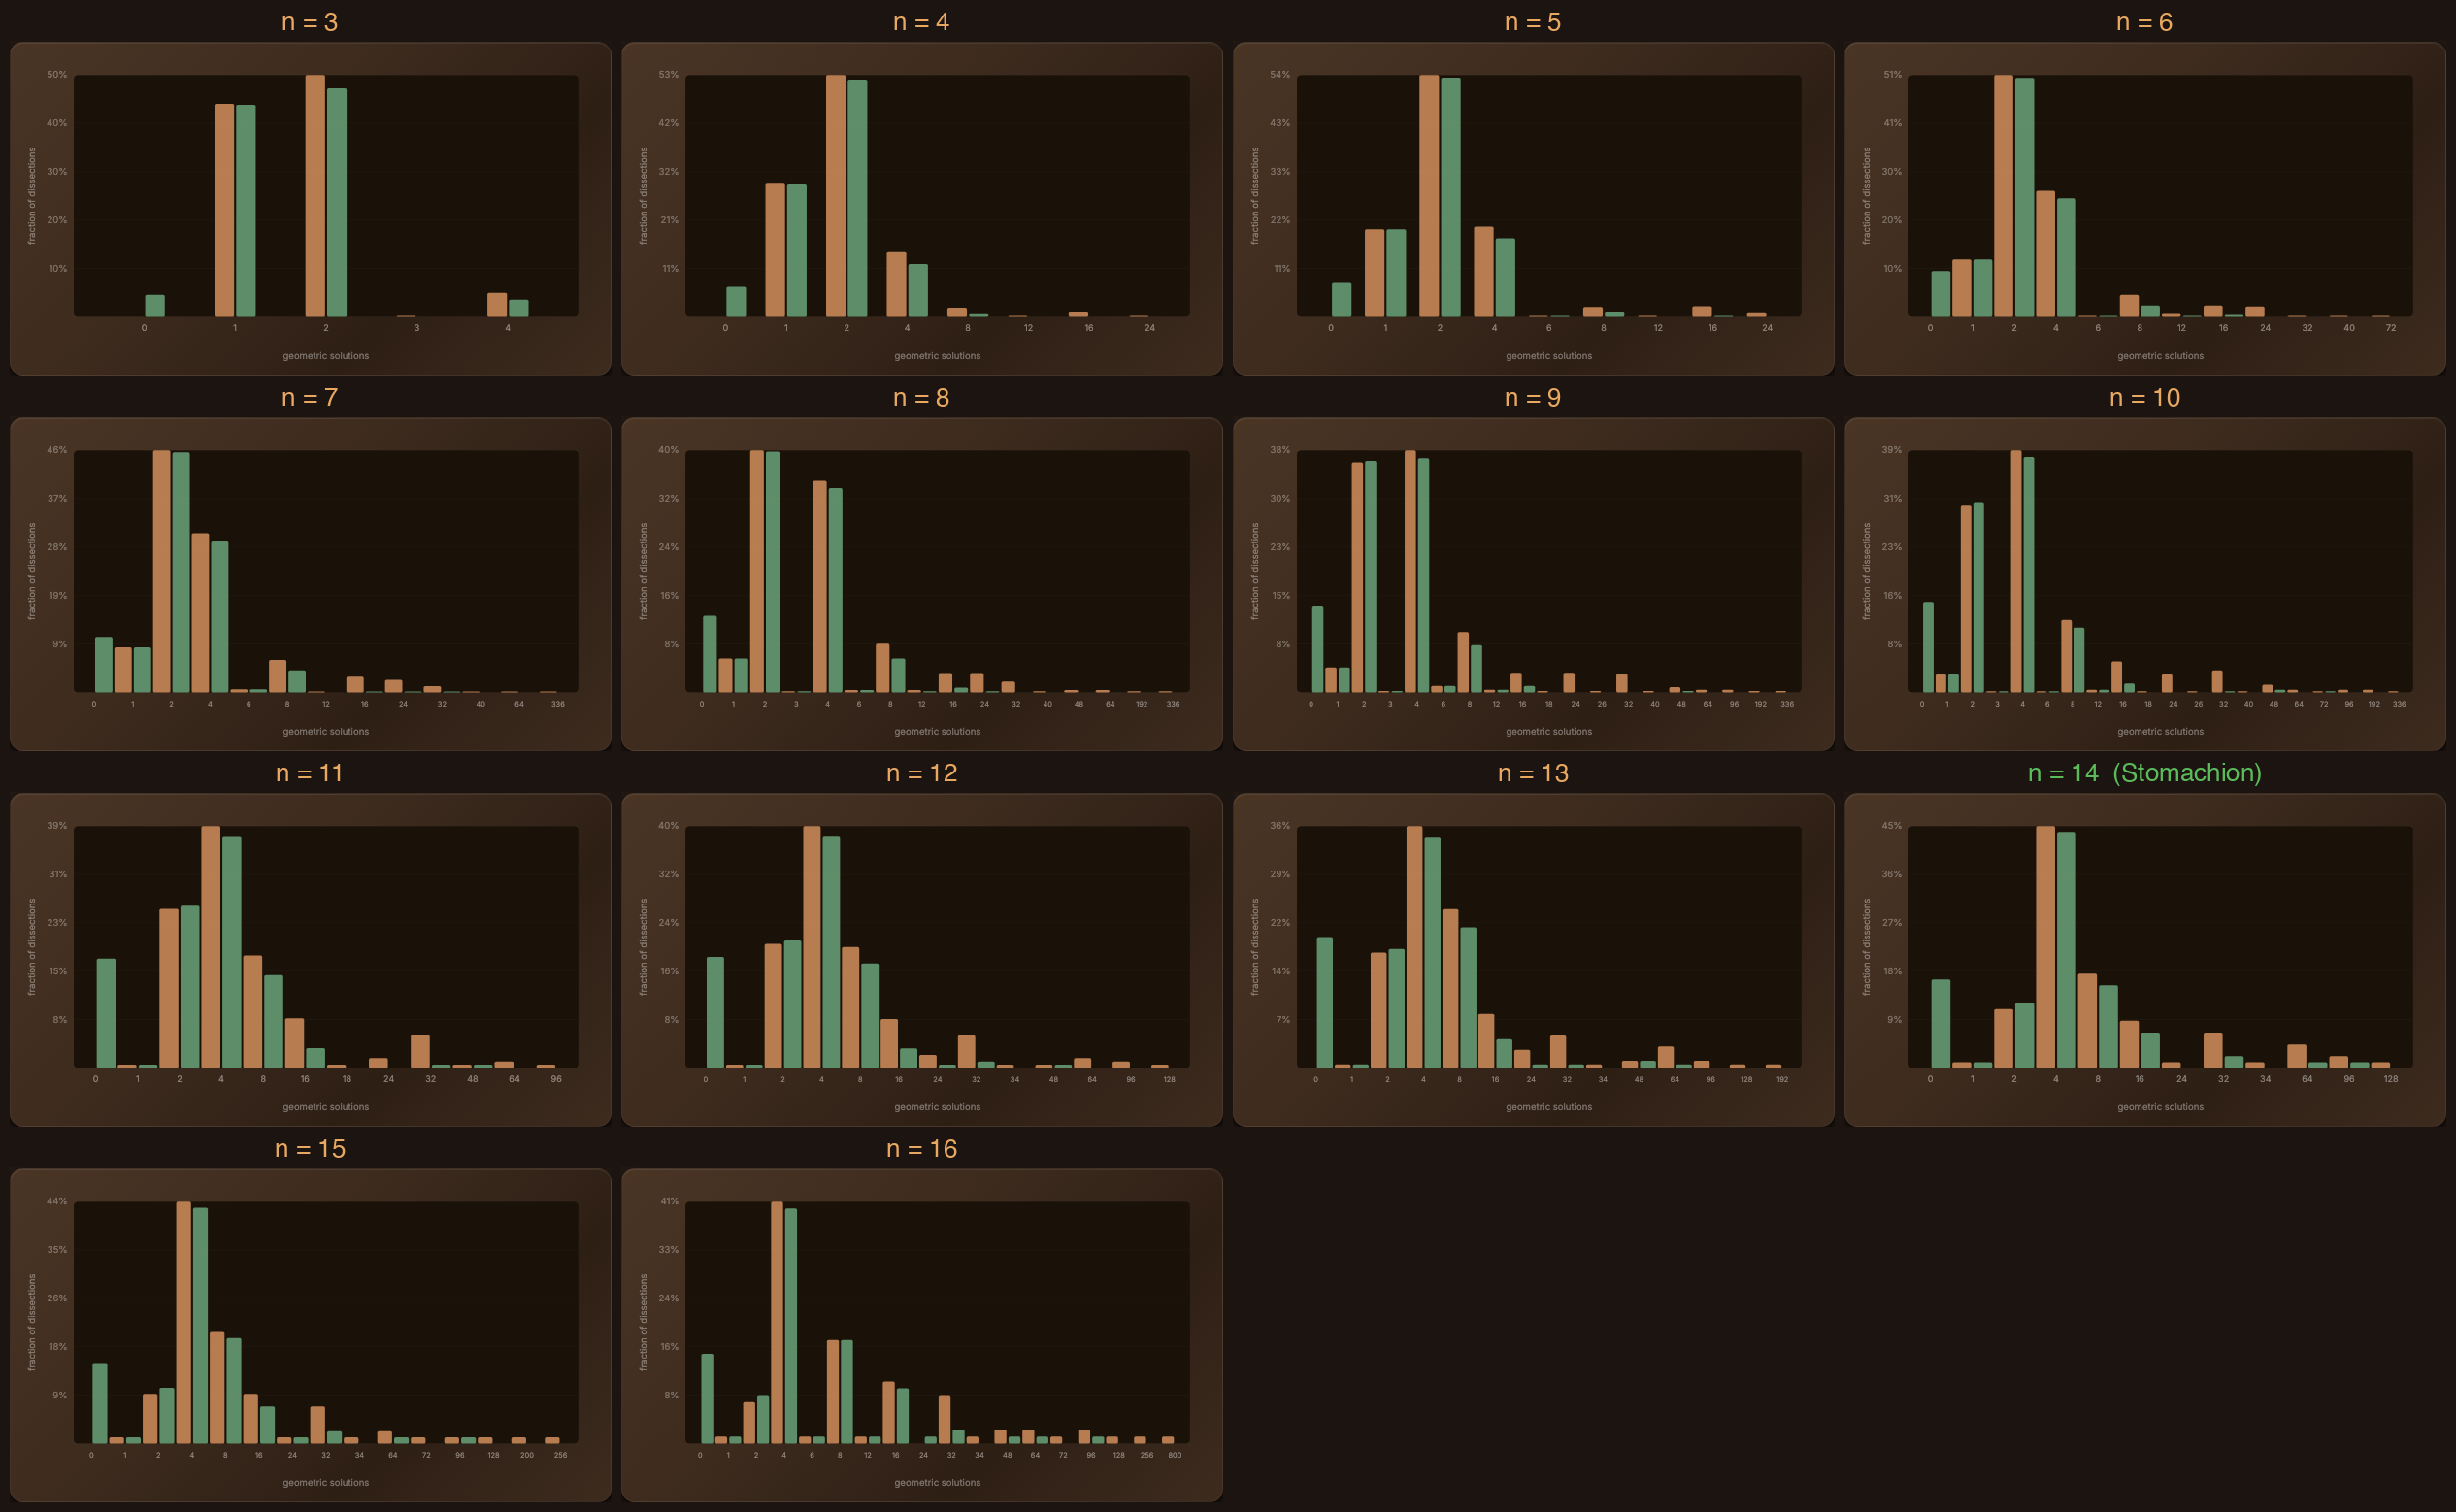
\includegraphics[width=\textwidth]{figures/histograms.png}
  \caption{Distribution of geometric tiling counts for random $n$-piece
    convex lattice dissections of the $12 \times 12$ square ($n = 3$ to
    $16$; $100$--$500$ trials per~$n$). Amber bars: total geometric
    tilings. Green bars: irreducible (fault-free) tilings only.
    The $n = 14$ panel (Stomachion's piece count, highlighted) shows a
    maximum of~$128$ from random sampling---the Stomachion's $2{,}144$ is
    completely off the chart. Note the concentration on powers of two
    and the growing gap between total and irreducible counts.}
  \label{fig:histograms}
\end{figure}

Several additional patterns are immediately apparent.

\begin{enumerate}[label=(\arabic*)]
\item \textbf{Rigidity is generic.}
  The fraction of rigid dissections ($\Sol = 1$) decreases as $n$
  grows, but a substantial majority of random dissections have at most
  $2$ tilings: $P(1) + P(2) > 70\%$ for $n \leq 7$. Rigidity is the
  norm; flexibility is the exception.

\item \textbf{Powers of two dominate.}
  Tiling counts of $1, 2, 4, 8, 16$ account for over $95\%$ of all
  dissections at every value of~$n$. Non-power-of-two counts (3, 6, 12,
  24, etc.)\ occur but are rare. This concentration reflects the
  multiplicative structure of the coproduct decomposition: each
  independent pairwise exchange doubles the tiling count.

\item \textbf{The median transitions from $2$ to $4$.}
  Between $n = 7$ and $n = 8$, the median tiling count jumps from $2$
  to $4$---the ``typical'' random dissection acquires its second
  independent exchange move around this point.

\item \textbf{Mean grows roughly linearly.}
  The mean tiling count grows approximately as $0.9n$, consistent with
  a linear increase in the expected number of independent exchange
  moves.

\item \textbf{A persistent maximum of 336.}
  For $n \geq 7$, the maximum observed tiling count is $336$ in every
  sample. This appears to be a single high-symmetry dissection
  (or family of dissections) that the random generator discovers across
  different values of~$n$.
\end{enumerate}

\begin{figure}[ht]
  \centering
  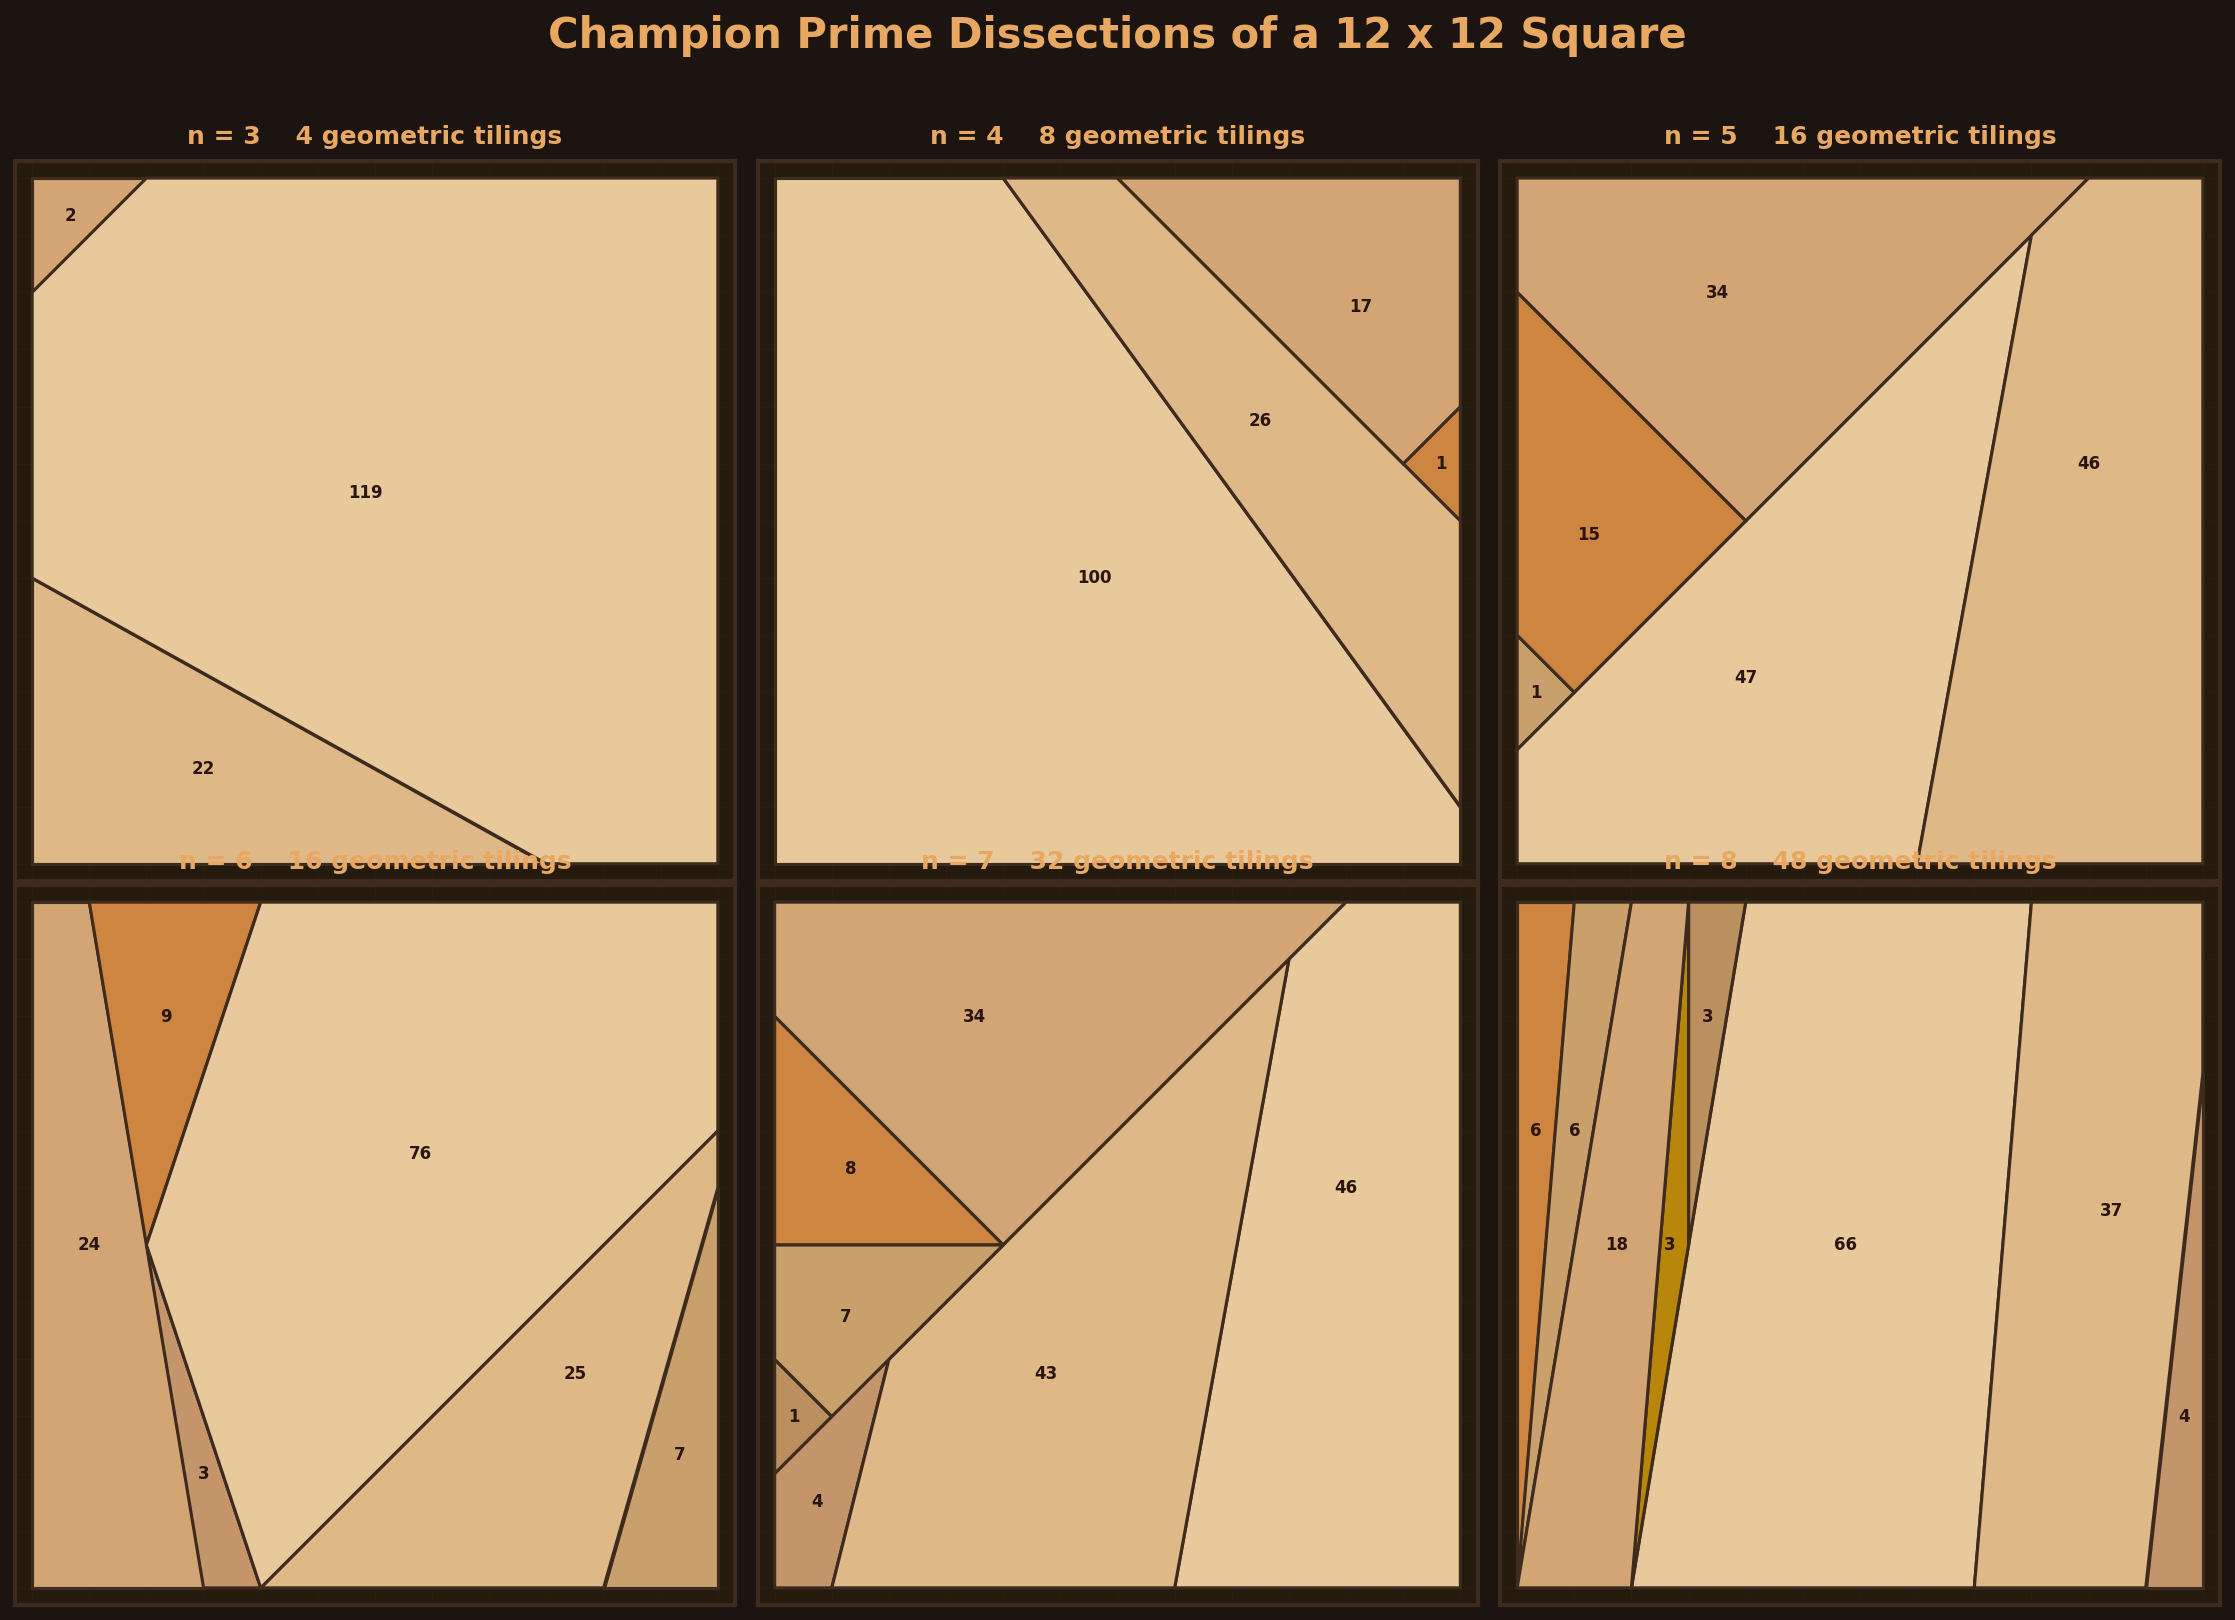
\includegraphics[width=0.85\textwidth]{figures/champions.png}
  \caption{Champion prime dissections for $n = 3$ through $n = 8$.
    Numbers inside each piece indicate area. All champions are generated
    by sequential lattice-point cuts, producing only convex pieces.
    Note the increasingly unbalanced piece distributions: each champion
    has a dominant piece ($\geq 30\%$ of area) with small satellites.}
  \label{fig:champions}
\end{figure}

\subsection{Reducible dissections easily beat 536}
\label{sec:reducible}

To demonstrate that the Stomachion's tiling count is not maximal among
\emph{all} 14-piece dissections, we conducted a simple search over
reducible dissections.

We placed a horizontal fault line at $y = 6$, dividing the $12 \times 12$
square into two $12 \times 6$ rectangles, and generated random $7$-piece
convex lattice dissections of each half independently. The total tiling
count of the composite dissection is the product of the two half-counts.

In $50$ random trials, the ninth trial produced a dissection with
$192 \times 24 = \mathbf{4{,}608}$ geometric tilings---roughly $9$ times
the Stomachion's $536$ (or about $2.1$ times its $2{,}144$). This
demonstrates that the multiplicative power of fault lines easily
overwhelms the flexibility of any single prime factor.

\begin{remark}
The reducible dissections in this experiment use only convex pieces,
while the Stomachion includes non-convex pieces (a pentagon and irregular
quadrilaterals). The comparison is thus between different classes of
dissection, but the qualitative point stands: reducibility is a far more
efficient route to high tiling counts than irreducible flexibility.
\end{remark}

\subsection{Champion prime dissections}
\label{sec:champions}

Having established that reducible dissections can trivially surpass the
Stomachion, the interesting question becomes: what is the maximum tiling
count among \emph{prime} dissections with $n$~pieces?

\begin{definition}[Champion]
A \emph{champion prime dissection} at~$n$ is an irreducible $n$-piece
lattice dissection of the $12 \times 12$ square achieving the maximum
geometric tiling count among all such dissections.
\end{definition}

\begin{table}[ht]
\centering
\caption{Champion prime dissections: maximum geometric tiling count
  among irreducible $n$-piece lattice dissections of the $12 \times 12$
  square. Values for $n \leq 6$ are from exhaustive or near-exhaustive
  search; values for $n \geq 7$ are lower bounds from random sampling.
  The Stomachion entry at $n = 14$ is marked with~$\star$.}
\label{tab:champions}
\medskip
\begin{tabular}{@{}c r l@{}}
\toprule
$n$ & Max prime count & Notes \\
\midrule
 3 &     1 & Near-exhaustive \\
 4 &     2 & Near-exhaustive \\
 5 &     4 & Near-exhaustive \\
 6 &     4 & Near-exhaustive \\
 7 &     8 & Random sampling lower bound \\
 8 &    24 & Random sampling lower bound \\
 9 &    48 & Random sampling lower bound \\
10 &   224 & Random sampling lower bound \\
11 &   120 & Random sampling lower bound \\
12 &   120 & Random sampling lower bound \\
13 &   120 & Random sampling lower bound (100\% irreducible) \\
\midrule
14 & 2{,}144 & Stomachion${}^\star$ (prime, verified; 32 irreducible) \\
\bottomrule
\end{tabular}
\end{table}

Figure~\ref{fig:n13champion} shows 16 of the 120 tilings of the
$n = 13$ champion. Despite having nearly as many pieces as the
Stomachion, this dissection is visually degenerate: it consists almost
entirely of long, thin triangles converging to a point, with no
resemblance to the balanced, ``designed'' feel of the Stomachion.
Yet every one of its 120~tilings is irreducible. The contrast
underscores that high tiling counts among prime dissections can arise
from very different geometric mechanisms.

\begin{figure}[ht]
  \centering
  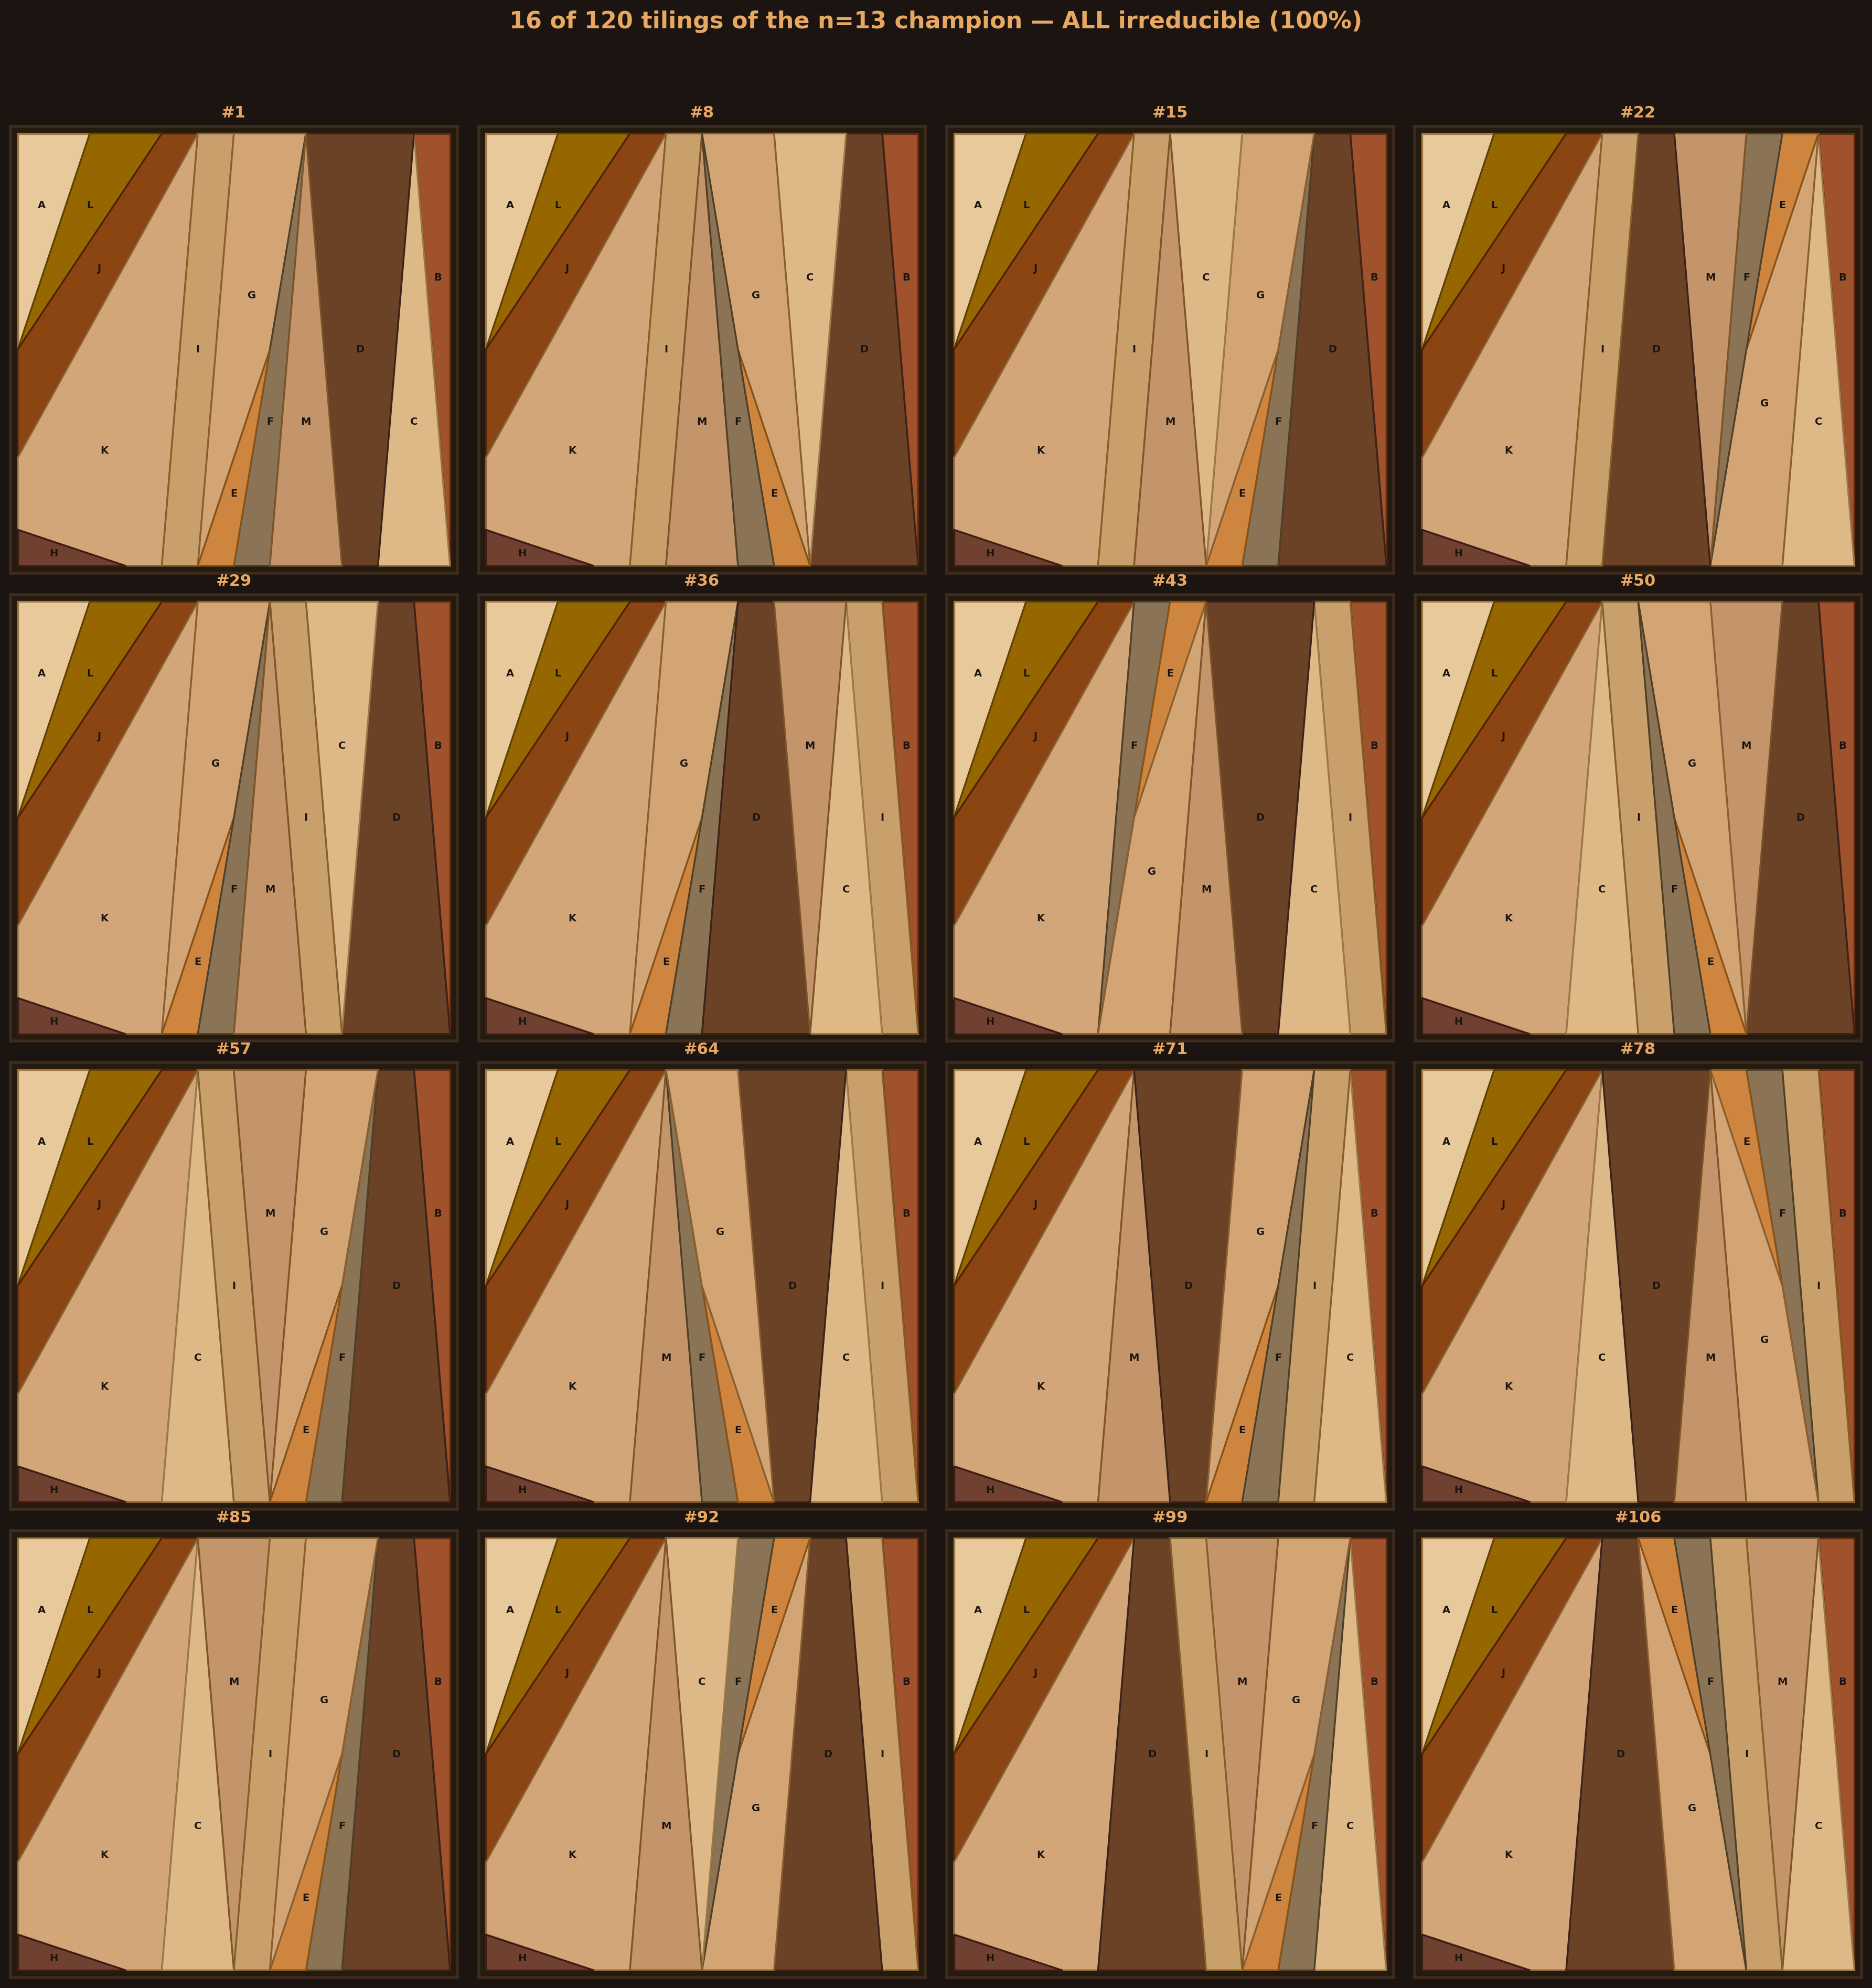
\includegraphics[width=0.75\textwidth]{figures/n13_champion.png}
  \caption{Sixteen of the 120~tilings of the $n = 13$ champion prime
    dissection---all irreducible. The dissection consists of long, thin
    triangles converging near a corner, producing high flexibility through
    edge-length coincidences despite its visually degenerate geometry.
    Compare with the balanced structure of the Stomachion
    (Figure~\ref{fig:stomachion}).}
  \label{fig:n13champion}
\end{figure}

The gap between the random-sampling champions at $n = 10$ (at most~$336$)
and the Stomachion at $n = 14$ ($2{,}144$) is enormous---a factor of
$6.4$. This gap likely reflects both the four additional pieces available
to the Stomachion and the limitations of the convex-piece random
generator, which cannot produce the non-convex pieces (pentagon,
irregular quadrilaterals) that the Stomachion employs.

\begin{conjecture}[Maximality of the Stomachion]
\label{conj:maximal}
Among all prime lattice dissections of the $12 \times 12$ square into
$14$ pieces, the Stomachion achieves the maximum geometric tiling count
of $2{,}144$.
\end{conjecture}

We regard this conjecture as plausible but far from established. The
evidence is threefold:
\begin{enumerate}[label=(\alph*)]
\item No $14$-piece prime dissection with more tilings has been found
  in extensive random sampling (though the sampling is biased toward
  convex pieces).
\item The Stomachion's pieces are defined by the ``natural construction
  lines'' of the square (diagonals, midlines, and their intersections
  with integer-grid lines), which create a maximal number of
  edge-length coincidences---precisely the condition for exchange moves.
\item The extreme rarity of high-count dissections in the random
  distribution (Table~\ref{tab:distribution}) suggests that $2{,}144$
  lies many standard deviations into the tail.
\end{enumerate}

\subsection{The Stomachion in the tail}
\label{sec:tail}

To place the Stomachion's count in context, consider the random
distribution at $n = 10$ (the largest~$n$ in our sample, still four
pieces short of the Stomachion). The mean tiling count is $9.0$, and
the maximum observed is $336$. Even accounting for the four additional
pieces at $n = 14$ (which would bring the extrapolated mean to roughly
$9.0 + 4 \times 0.9 \approx 12.6$ by the linear trend), the
Stomachion's $2{,}144$ is roughly $170$ times the expected mean.

In terms of the exchange-move count $k$ (where the tiling count is
approximately $2^k$), the Stomachion has $k \approx \log_2(2144) \approx
11.1$. Under the Poisson model with $\lambda \approx 0.15$ and
$n = 14$, the expected number of exchange moves is
$\lambda n \approx 2.1$, so $k = 11$ corresponds to a
fluctuation of roughly $9$ moves above the mean---an event of
probability $\approx 2.1^{11}/11! \approx 5 \times 10^{-5}$ under
the Poisson law. The Stomachion is a $4$--$5$ sigma outlier.

\subsection{Fault-line anatomy of the Stomachion}
\label{sec:anatomy}

Applying the forced/optional fault-line analysis of
Section~\ref{sec:verification} to each of the $17{,}152$ raw
solutions individually reveals a striking decomposition. We checked
every solution for optional fault lines along $y = k$, $x = k$
($k = 1, \ldots, 11$) and the diagonals $y = x$, $y = 12 - x$.

\begin{table}[ht]
\centering
\caption{Fault-line structure of the Stomachion's $536$ tilings
  (Cutler equivalence). A solution ``has'' a fault line if all
  $14$~pieces in that tiling lie entirely on one side of it.}
\label{tab:anatomy}
\medskip
\begin{tabular}{@{}l r r@{}}
\toprule
Category & Tilings & Fraction \\
\midrule
Fault-free (no optional fault line) &  32 &  6\% \\
Exactly one fault line              & 496 & 93\% \\
Two or more fault lines             &   8 &  1\% \\
\midrule
Total (Cutler)                      & 536 & 100\% \\
\bottomrule
\end{tabular}
\end{table}

The optional fault lines that appear are precisely the natural
construction lines: $y = 6$ (horizontal midline) appears in $46\%$ of
solutions, $x = 6$ (vertical midline) in $46\%$, and the two diagonals
$y = x$ and $y = 12 - x$ each in approximately $1.5\%$.

This reveals that the Stomachion's high tiling count arises predominantly
from its \emph{optional} coproduct structure: in most tilings, the
pieces happen to align along a midline, creating a temporary
decomposition into two independent halves. The $32$ fault-free tilings
form the irreducible core---the configurations where all $14$~pieces
are genuinely interlocked with no line of separation.

\begin{figure}[p]
  \centering
  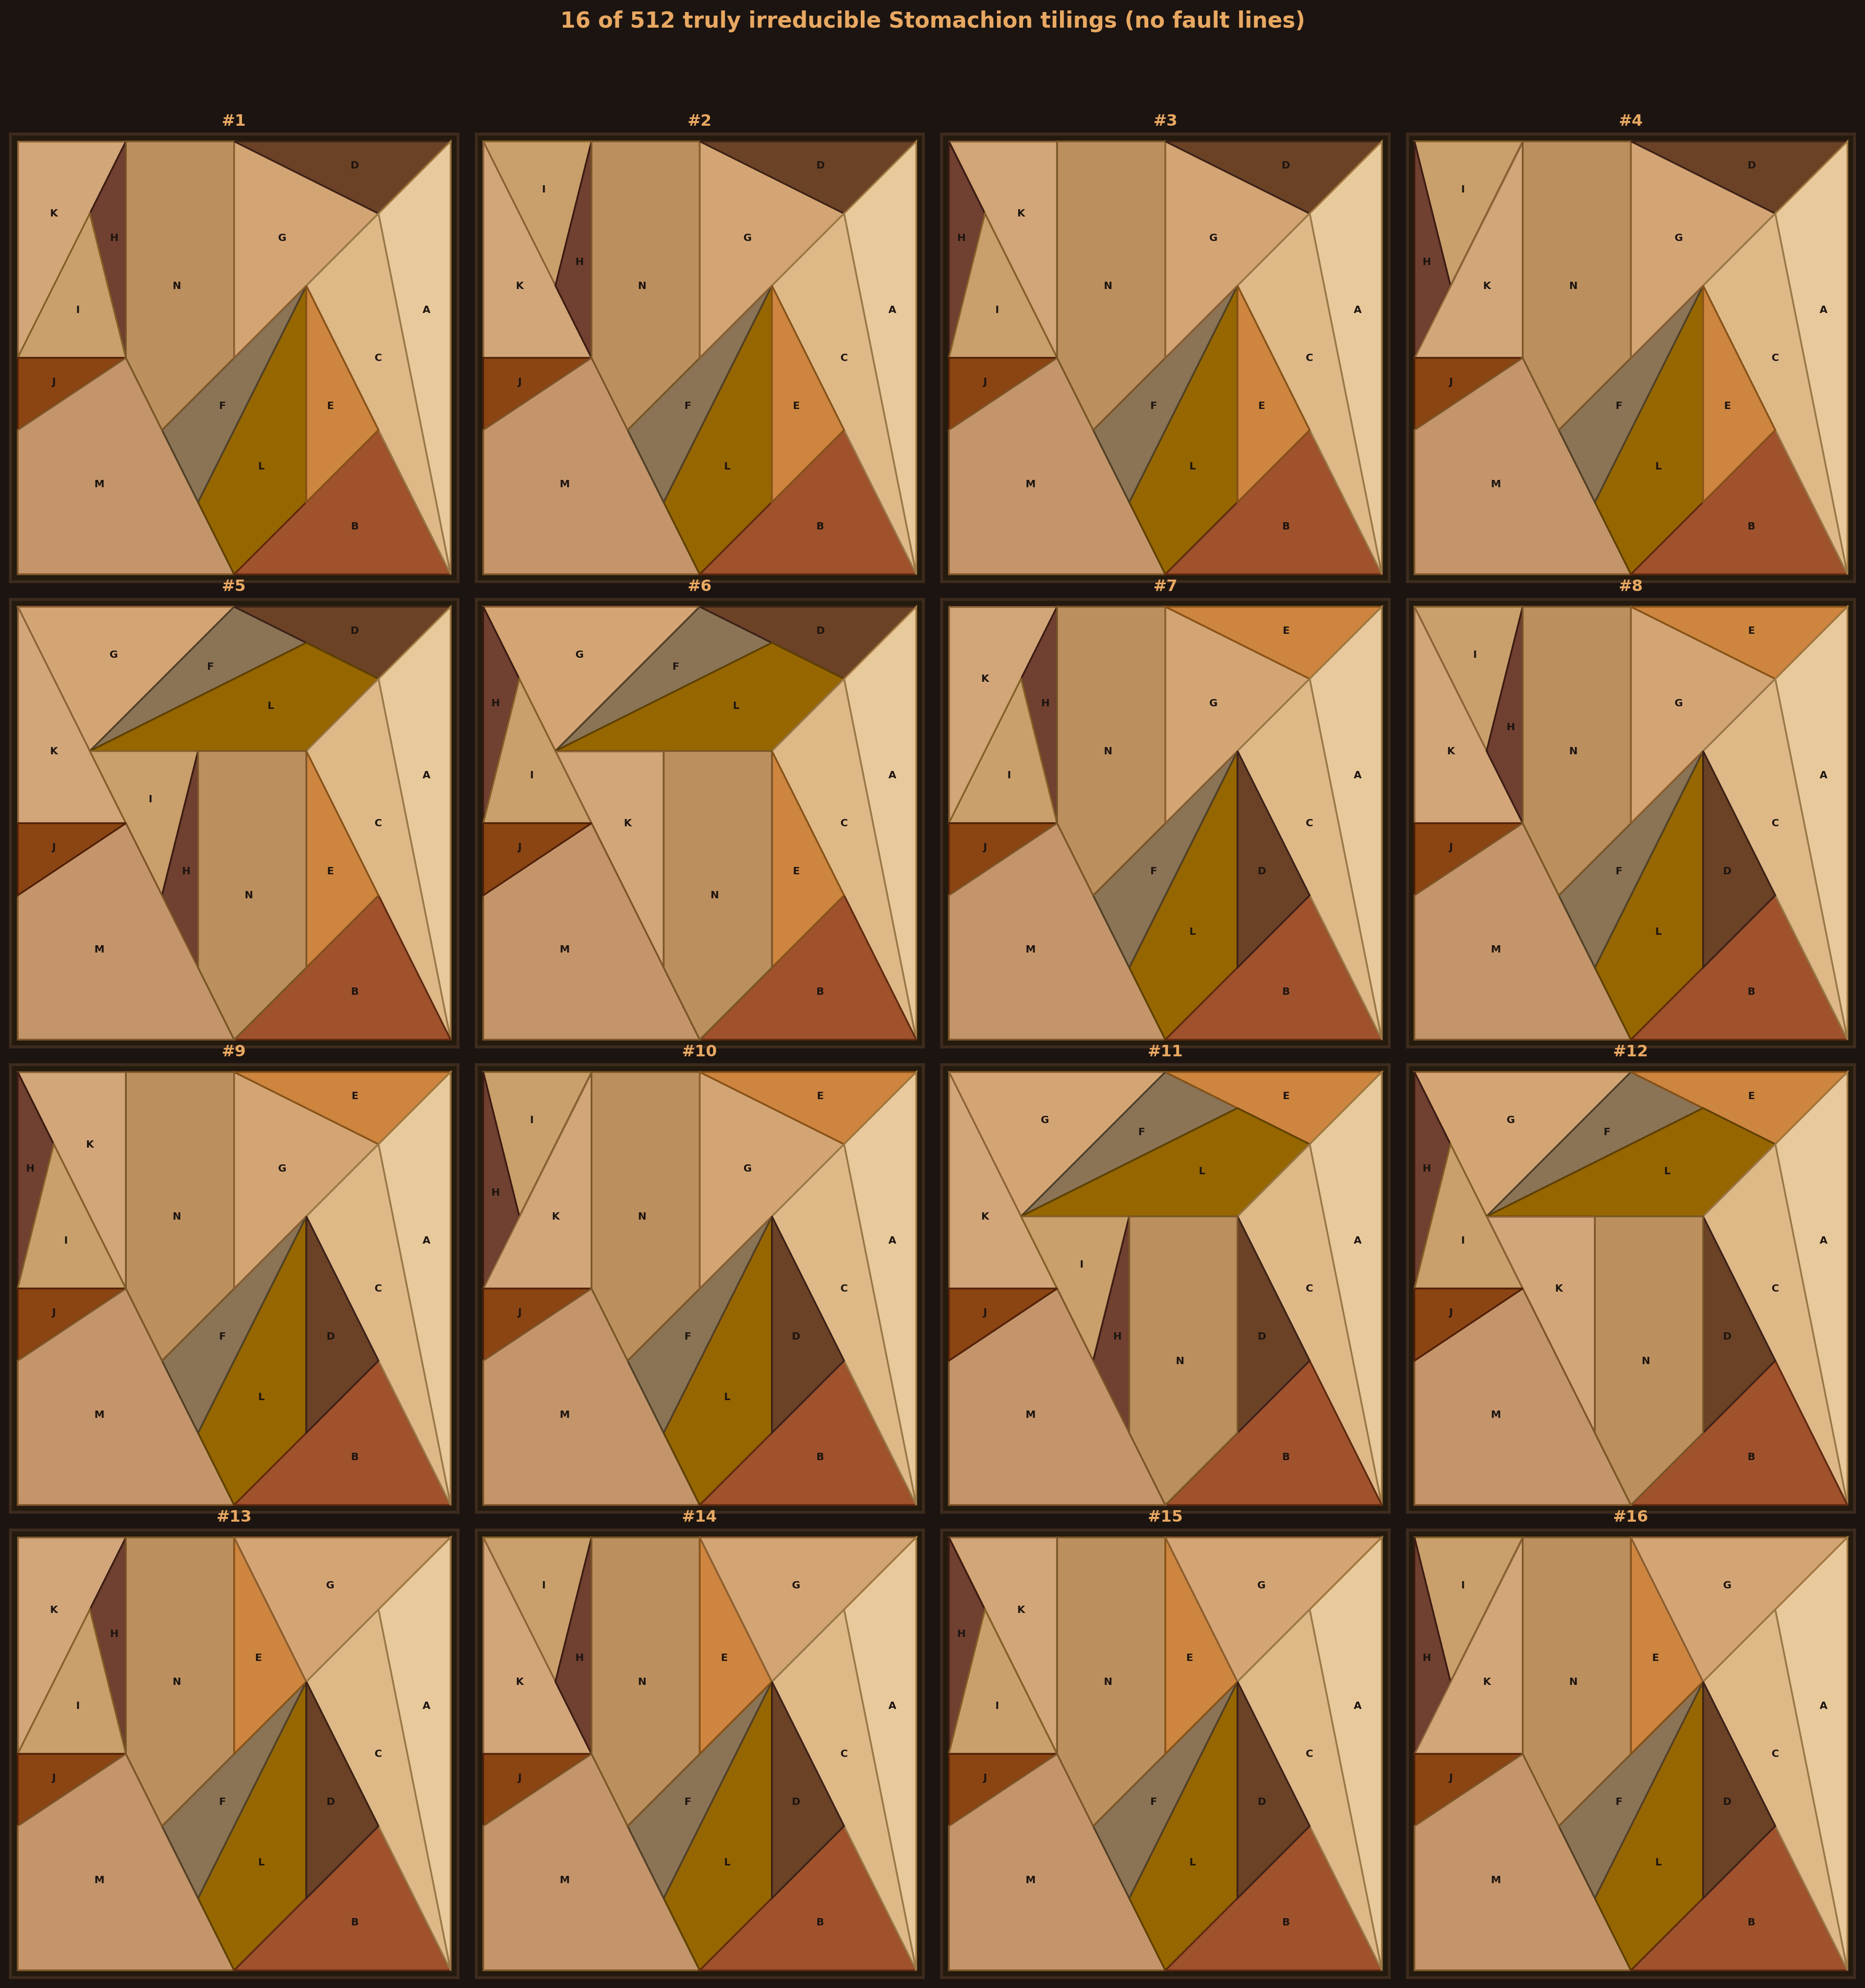
\includegraphics[width=0.92\textwidth]{figures/stomachion_irreducible.png}
  \caption{Irreducible Stomachion tilings \#1--16 (of 32 total). No
    straight line from boundary to boundary separates the pieces.}
  \label{fig:irreducible_a}
\end{figure}

\begin{figure}[p]
  \centering
  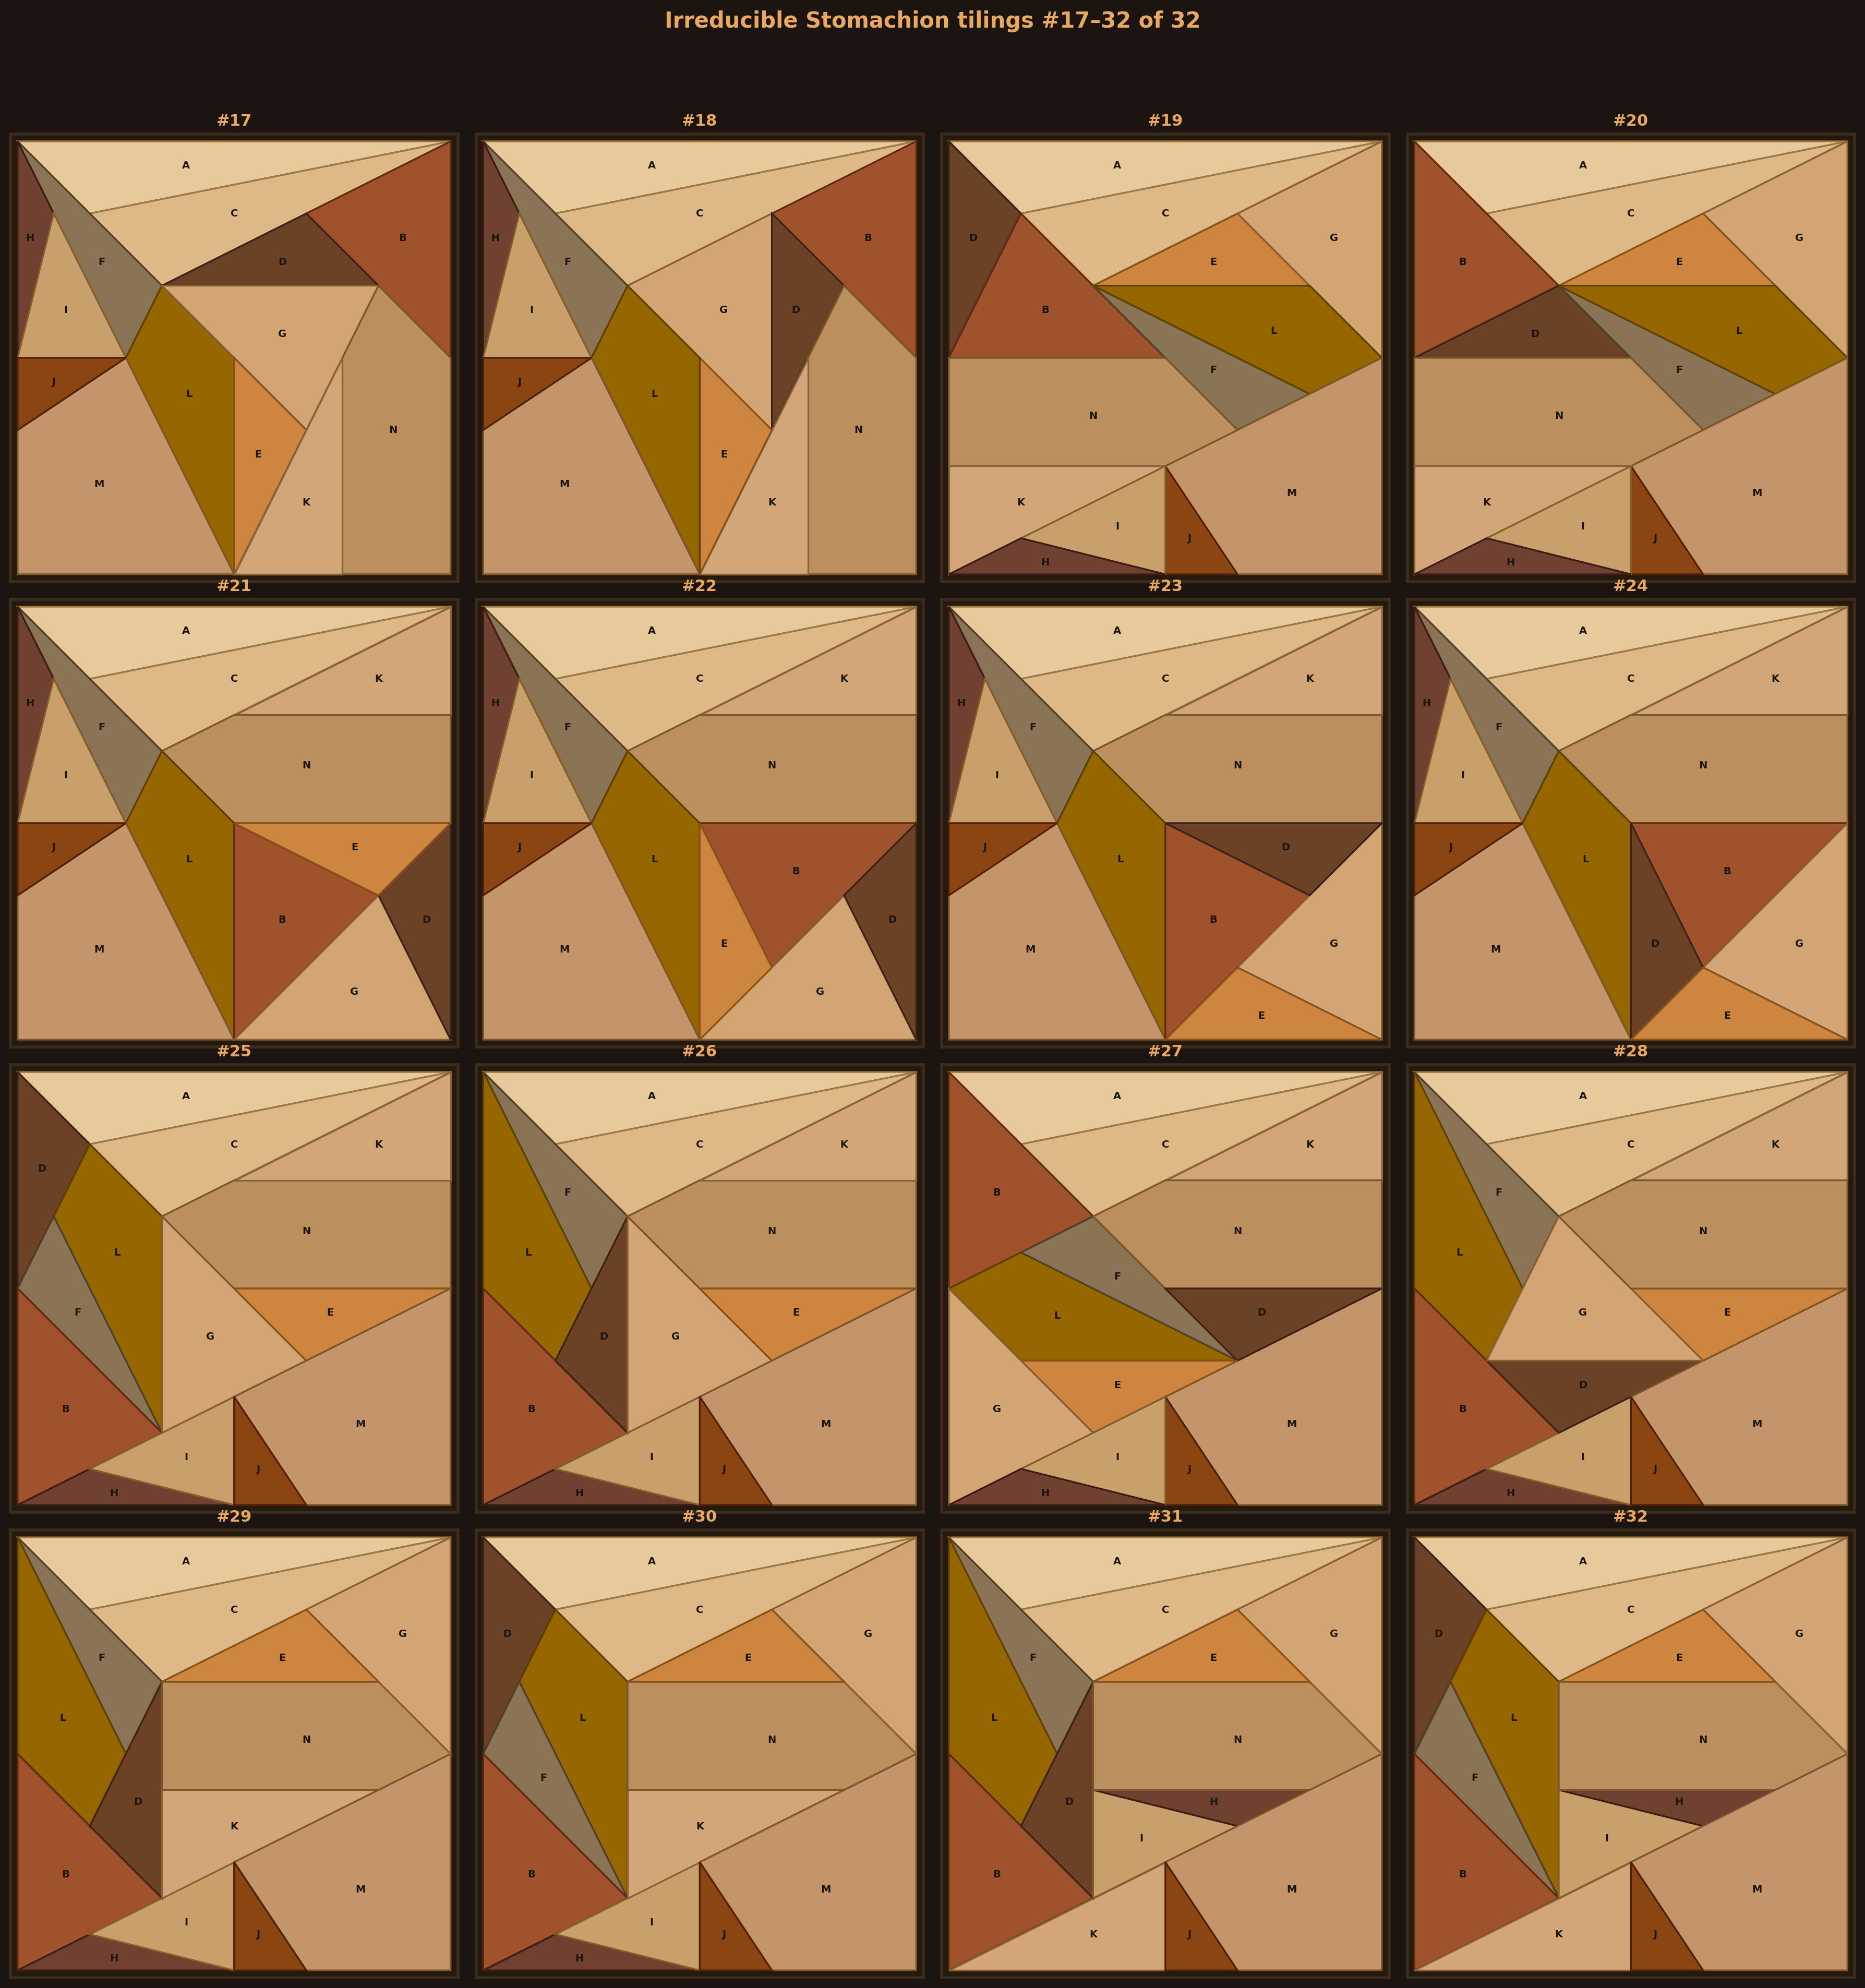
\includegraphics[width=0.92\textwidth]{figures/stomachion_irreducible_2.png}
  \caption{Irreducible Stomachion tilings \#17--32. Together with
    Figure~\ref{fig:irreducible_a}, these are all $32$ fault-free tilings
    of the Stomachion. Every piece occupies genuinely different positions
    across the $32$ configurations.}
  \label{fig:irreducible_b}
\end{figure}

\subsection{The $n = 13$ champion: a counterpoint}
\label{sec:n13}

Our random search found an $n = 13$ prime dissection
(convex pieces, generated by sequential cuts) with $120$ distinct
tilings modulo~$\D_4$---all of them fault-free. This dissection is
$100\%$ irreducible: none of its solutions admit any optional fault line.

Surprisingly, this property is not rare. A scan of $200$ random
dissections at each~$n$ reveals that \emph{most} random dissections
are all-irreducible: the fraction rises from $50\%$ at $n = 3$
to $82\%$ at $n = 8$. What makes the $n = 13$ champion remarkable
is not its irreducibility (which is generic) but achieving $120$
tilings while maintaining it. The best all-irreducible dissections
found by random search top out at $16$~tilings for $n \leq 8$.

On the irreducible metric alone, this champion surpasses the Stomachion
($120 > 32$). However, it falls short on every other measure of puzzle
quality:

\begin{center}
\begin{tabular}{@{}l c c@{}}
\toprule
Property & $n = 13$ champion & Stomachion \\
\midrule
Total tilings ($\D_4$) & 120 & 2{,}144 \\
Irreducible tilings & 120 (100\%) & 32 (6\%)\footnotemark \\
Piece participation & 7/13 mobile & 14/14 mobile \\
Largest piece & 21\% of area & 17\% of area \\
Shape diversity & all triangles & $11\triangle\; 2\square\; 1\pentagon$ \\
\bottomrule
\end{tabular}
\end{center}
\footnotetext{Using the $\D_4$-only equivalence with $2{,}144$ total;
under Cutler equivalence, $32/536 = 6\%$.}

The champion's $120$ tilings, though all irreducible, involve only
$7$ of its $13$ pieces---the remaining $6$ (comprising $41\%$ of the
area) are frozen in place across all configurations. By contrast,
the Stomachion moves all $14$ pieces: with $2{,}144$ tilings, it is
impossible for any single piece (at most $17\%$ of the area) to remain
fixed.

\begin{figure}[ht]
  \centering
  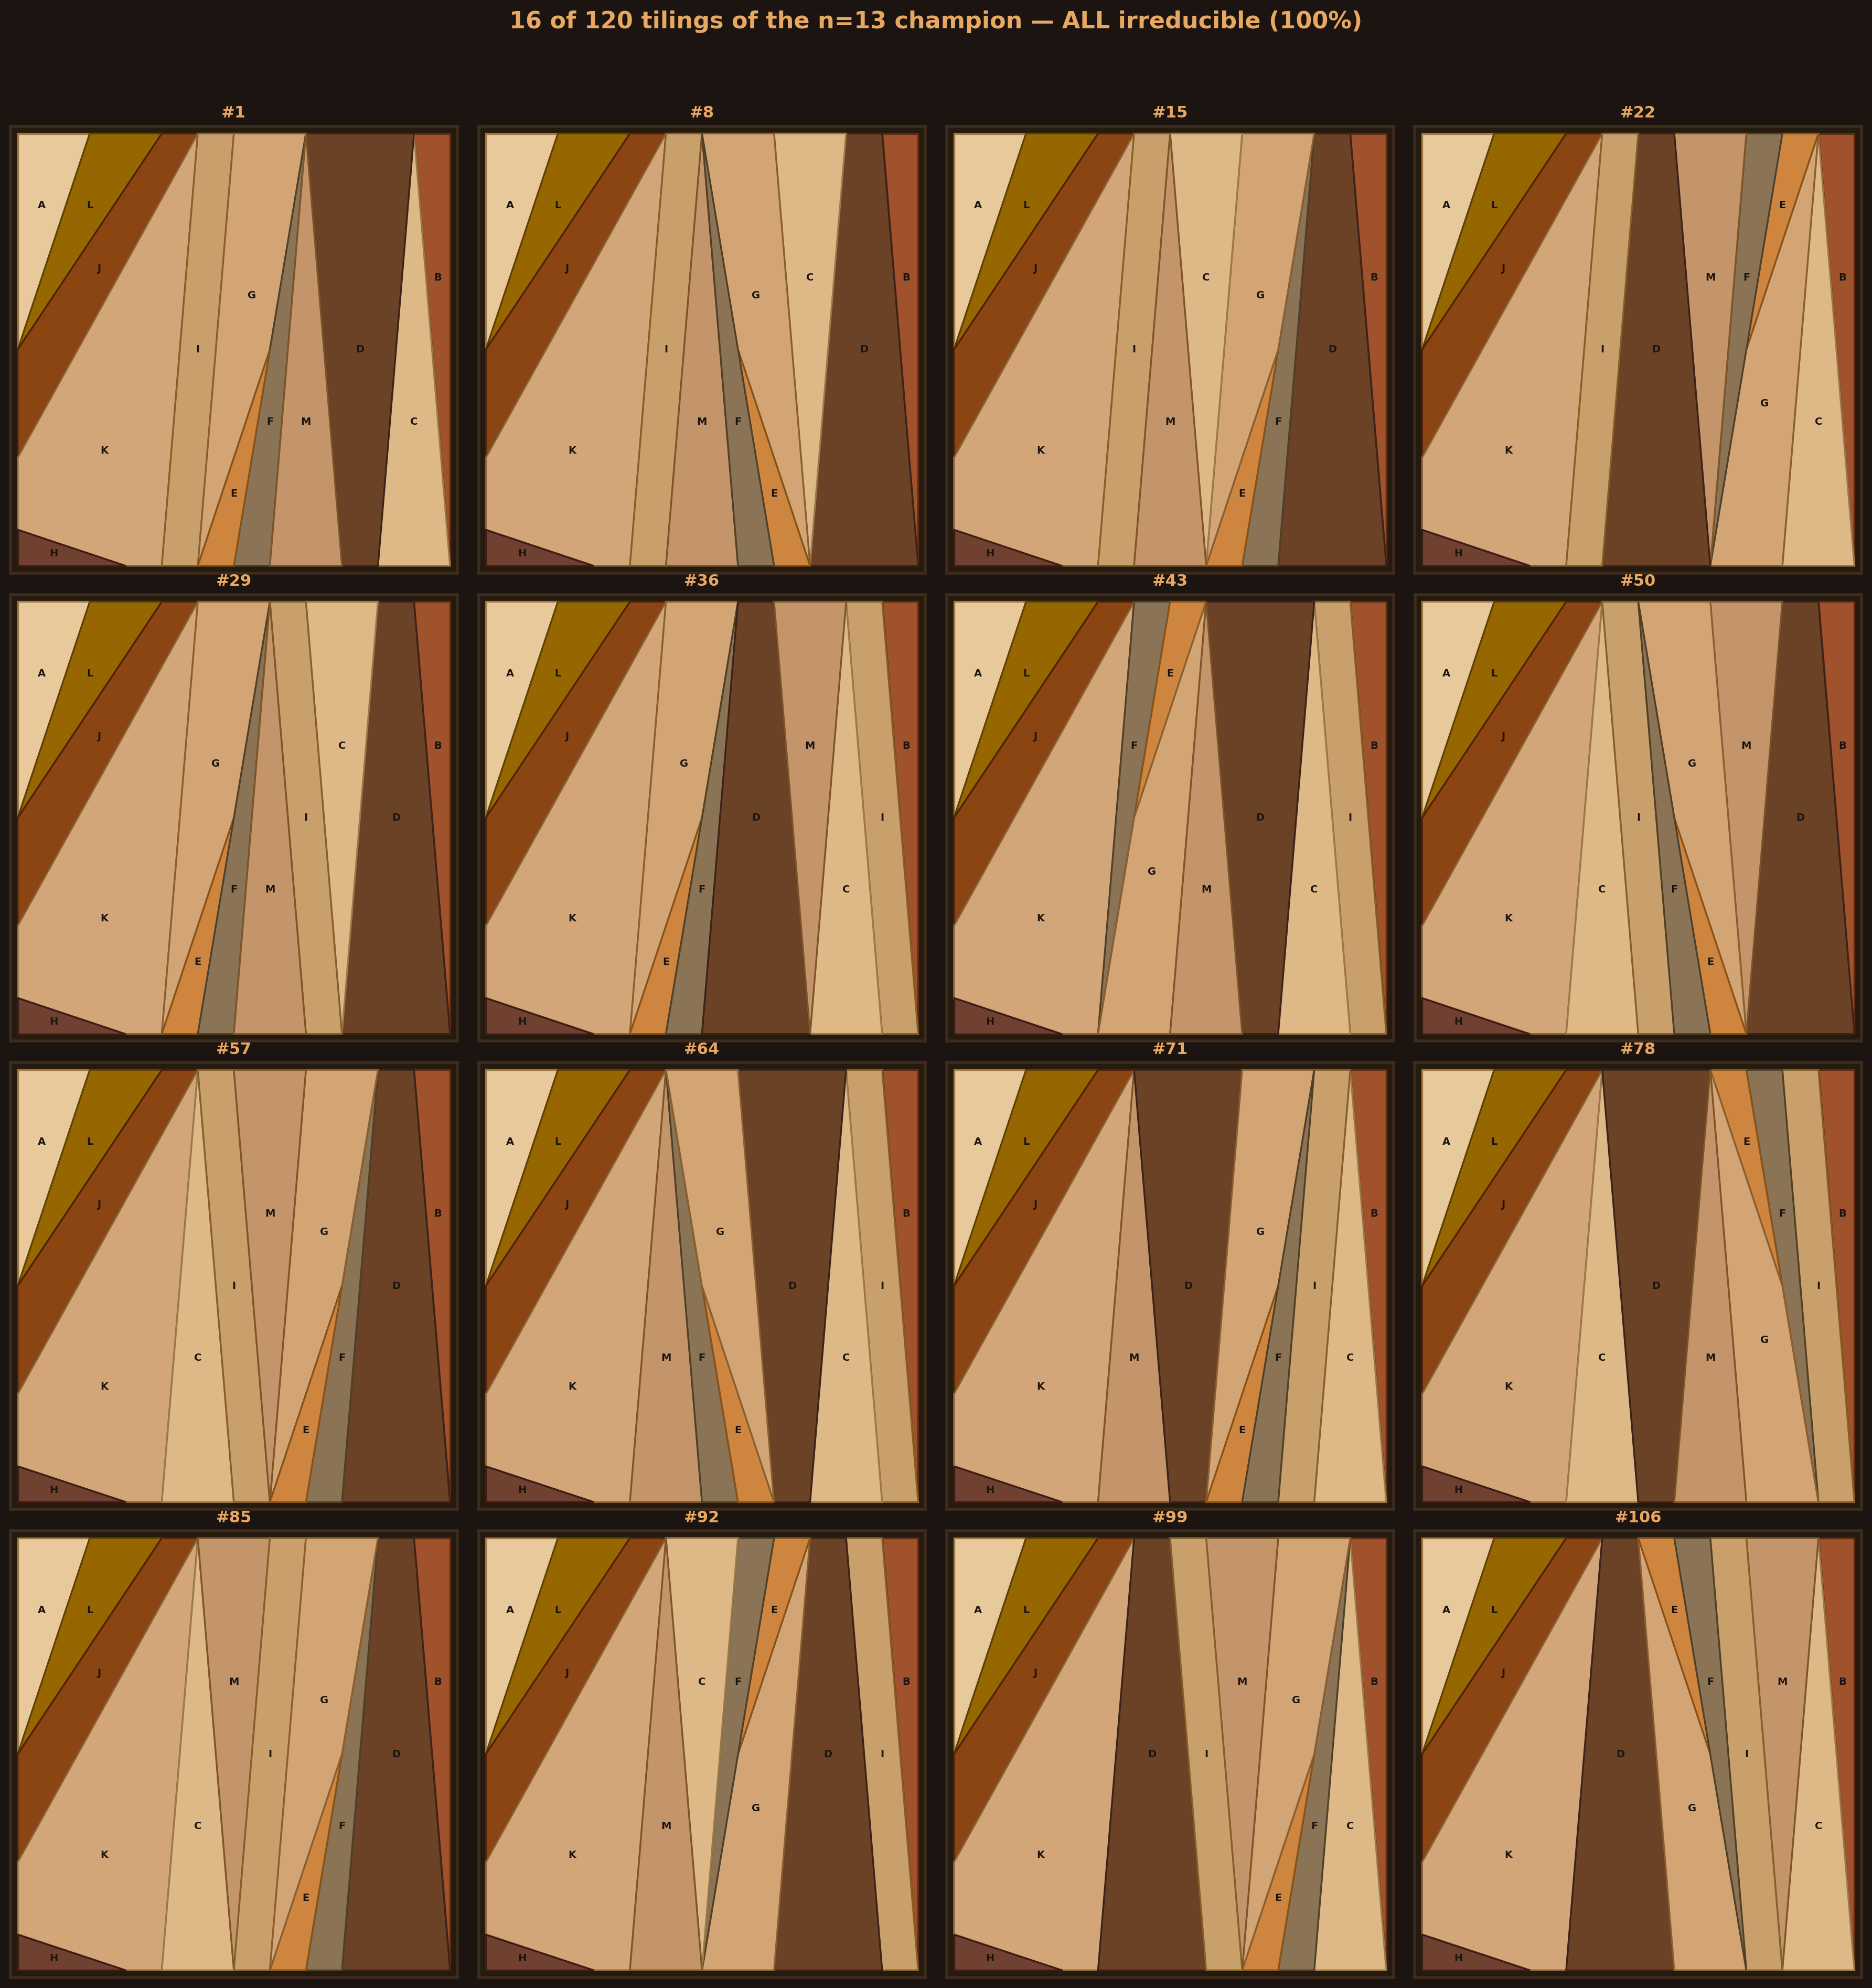
\includegraphics[width=0.9\textwidth]{figures/n13_champion.png}
  \caption{Sixteen of the $120$ tilings of the $n = 13$ champion prime
    dissection. All $120$ are irreducible (no optional fault lines),
    but only $7$ of $13$ pieces participate---the remaining $6$ are
    frozen in place. The pieces are all elongated convex triangles,
    lacking the shape diversity of the Stomachion.}
  \label{fig:n13}
\end{figure}

\subsection{The multi-axis view}
\label{sec:multiaxis}

No single metric captures what makes the Stomachion special. The
dissections that beat it on any one axis invariably fail on the others:

\begin{enumerate}[label=(\roman*)]
\item \textbf{Total tilings.} Reducible dissections with a single
  fault line achieve $4{,}608$---but they are ``two puzzles glued
  together,'' not a single coherent design.
\item \textbf{Irreducible tilings.} The $n = 13$ random champion
  achieves $120$ fault-free tilings, beating the Stomachion's $32$---but
  with frozen pieces, unbalanced areas, and no shape variety.
\item \textbf{Balance and participation.} These emerge naturally
  at $n \geq 10$ in random search, but always with low tiling counts.
\end{enumerate}

There is also an axis that resists quantification:
\emph{aesthetic quality}. The Stomachion's pieces arise from the natural
construction lines of the square---diagonals, midlines, and their
intersections---producing shapes with visual harmony and a pleasing
variety of triangles, quadrilaterals, and a pentagon
(Figure~\ref{fig:stomachion}). The champion primes found by random
search are, without exception, visually unappealing: elongated slivers,
lopsided triangles, no diversity of shape (Figures~\ref{fig:champions}
and~\ref{fig:n13}). They achieve flexibility through geometric
coincidence but not through geometric elegance.

The Stomachion appears to be the unique dissection that scores
well on \emph{all} axes simultaneously: high total count, nontrivial
irreducible core, full participation, balanced piece sizes,
diversity of piece shapes, and aesthetic coherence. It achieves this
through the elegant mechanism of optional fault lines: the natural
construction lines of the square create a web of potential
decompositions that collectively generate $536$ tilings, of which $32$
are genuinely irreducible and all $14$ pieces participate across the
full solution space.

%% ===================================================================
\section{The Poisson Conjecture}
\label{sec:poisson}
%% ===================================================================

The concentration of tiling counts on powers of two suggests a simple
generative model: each tiling arises from a collection of
\emph{independent exchange moves}, each of which doubles the count.

\begin{definition}[Exchange move]
An \emph{exchange move} in a dissection is a subset of pieces that can be
rearranged (within their collective footprint) in exactly two ways while
the remaining pieces stay fixed. Two exchange moves are
\emph{independent} if they involve disjoint sets of pieces occupying
disjoint regions of the square.
\end{definition}

If a dissection has $k$ independent exchange moves, then its tiling
count is $2^k$ (each move can be independently toggled). Non-power-of-two
counts arise from exchange moves that are not fully independent, or from
moves with more than two states.

\begin{conjecture}[Poisson law for exchange moves]
\label{conj:poisson}
For a random $n$-piece convex lattice dissection of the $12 \times 12$
square (generated by the sequential-cut process), the number of
independent exchange moves $k$ satisfies
\[
k \;\approx\; \mathrm{Poisson}(\lambda n)
\]
for a constant $\lambda \approx 0.15$, as $n \to \infty$ on the integer
grid.
\end{conjecture}

\textbf{Evidence.} The observed fraction of rigid dissections ($k = 0$)
provides the strongest test. Under a Poisson model,
$P(k = 0) = e^{-\lambda n}$. The observed values are:

\begin{table}[ht]
\centering
\caption{Comparison of observed rigidity fraction $P(1)$ with the
  Poisson prediction $e^{-\lambda n}$ for $\lambda = 0.15$.}
\label{tab:poisson_fit}
\medskip
\begin{tabular}{@{}c c c@{}}
\toprule
$n$ & Observed $P(\text{rigid})$ & $e^{-0.15n}$ \\
\midrule
 3 & 0.44 & 0.64 \\
 4 & 0.29 & 0.55 \\
 5 & 0.20 & 0.47 \\
 6 & 0.12 & 0.41 \\
 7 & 0.09 & 0.35 \\
 8 & 0.06 & 0.30 \\
 9 & 0.04 & 0.26 \\
10 & 0.03 & 0.22 \\
\bottomrule
\end{tabular}
\end{table}

The Poisson model with $\lambda = 0.15$ consistently overestimates the
rigidity fraction, suggesting that the true decay is faster than
$e^{-0.15n}$---perhaps $\lambda$ is somewhat larger, or the Poisson
approximation is rough. A better fit might be obtained with
$\lambda \approx 0.25$--$0.30$ (which gives $e^{-0.25 \cdot 10}
\approx 0.08$, closer to the observed $0.03$), or by allowing $\lambda$
to depend weakly on~$n$. We retain $\lambda \approx 0.15$ as a
conservative estimate consistent with the mean growth rate
($\mathbb{E}[2^k] \approx 0.9n$ requires $\mathbb{E}[k] \approx
\log_2(0.9n)$, which is sublinear), though the full picture is likely
more subtle.

\textbf{Connection to the Chen-Stein method.}
The Poisson conjecture is amenable to analysis via the
\emph{Chen-Stein method}~\cite{ChenStein}, which provides bounds on the
total variation distance between the distribution of a sum of
weakly dependent indicator random variables and a Poisson distribution.
Here, each potential exchange move is an indicator variable
$X_i \in \{0, 1\}$, and $k = \sum_i X_i$. The Chen-Stein bound requires
estimating:
\begin{itemize}
  \item $b_1 = \sum_{i} \sum_{j \in N(i)} \mathbb{E}[X_i]\,
    \mathbb{E}[X_j]$, where $N(i)$ is the ``neighborhood'' of
    potential move~$i$ (those sharing pieces or area with~$i$),
  \item $b_2 = \sum_{i} \sum_{j \in N(i),\, j \neq i}
    \mathbb{E}[X_i X_j]$,
\end{itemize}
and showing that both are small relative to $\lambda = \sum_i
\mathbb{E}[X_i]$. The key difficulty is estimating these expectations
for random lattice dissections, where the geometry of piece boundaries
creates complex dependencies.

\textbf{The geometric count.}
Since the tiling count is approximately $2^k$ and $k$ is approximately
Poisson, the distribution of tiling counts is approximately
\emph{log-Poisson}: $\log_2(\text{count})$ is approximately Poisson.
This explains the concentration on powers of two and the exponentially
heavy right tail observed in Table~\ref{tab:distribution}. The
distribution is neither Gaussian (the tail is too heavy) nor truly
log-normal (the support is discrete and concentrated), but a
\emph{discrete log-Poisson}: a Poisson variable exponentiated to
base~$2$.

%% ===================================================================
\section{Discussion}
\label{sec:discussion}
%% ===================================================================

\subsection{Why Archimedes chose the Stomachion}

Our results suggest a compelling interpretation of Archimedes' puzzle.
The Stomachion is prime---no forced fault lines---yet its solution space
is extraordinarily rich, with $2{,}144$ geometric tilings. Among
random prime dissections of comparable size, this count is a
$4$--$5$ sigma outlier.

The source of this richness is not brute combinatorial complexity but
\emph{structural depth}. The Stomachion's solutions exhibit many
different optional fault-line patterns: some tilings decompose along
a diagonal, others along a different line, still others admit no fault
line at all. Each pattern contributes a multiplicative family of
solutions via the coproduct decomposition. The total count is a sum
of products---a rich coproduct structure arising from a prime dissection.

This stands in sharp contrast to the champion primes found by random
search (Section~\ref{sec:champions}), which achieve flexibility through
unbalanced piece distributions: one large inert piece with small
satellites shuffling around its edges. The Stomachion has no piece
larger than $17\%$ of the total area, and every piece participates
across all $2{,}144$ tilings. Its flexibility is \emph{distributed}
rather than \emph{localized}.

The Stomachion's pieces are defined by the natural construction lines of
the square: the two diagonals, the two midlines, and the lines
connecting vertices to midpoints of opposite sides. These construction
lines, when restricted to the integer lattice, create a dense web of
intersections and many edge-length coincidences---precisely the
conditions that enable both exchange moves and optional fault lines.

We speculate that Archimedes discovered the Stomachion not by searching
for a dissection with many solutions, but by noticing that the natural
construction lines of the square produce an unusually rich puzzle. The
combinatorial question---\emph{how many ways can the pieces tile the
square?}---may have been the original motivation for the lost treatise.

The fragment of the Archimedes Palimpsest that survives~\cite{Netz2004}
is tantalizing but incomplete. It contains the phrase ``the number of
figures,'' which Netz interprets as evidence that Archimedes was
interested in the enumeration problem. Our results support this
interpretation: the Stomachion is remarkable precisely because of the
combinatorial richness that emerges from its geometric simplicity.

\subsection{Physical puzzle interpretation}

From the perspective of puzzle design, our prime factorization theorem
provides a natural grading of difficulty. A reducible dissection is
``easy'' in the sense that it decomposes into independent sub-puzzles; a
prime dissection is ``hard'' because all pieces interact.

The sequence of champion primes---dissections achieving the maximum
tiling count at each~$n$---forms a natural family of wooden puzzles of
increasing complexity. At $n = 3$ or $n = 4$, the champion has only a
handful of solutions. At $n = 14$, the champion is (conjecturally) the
Stomachion, with $2{,}144$ solutions---a puzzle that is paradoxically
both ``easy'' (many solutions exist) and ``hard'' (the solution space is
large but the pieces are interlocked in complex ways).

This dual nature may explain the Stomachion's enduring appeal: it is
accessible enough that a patient solver will find solutions, yet rich
enough that the enumeration problem is genuinely deep.

\subsection{Open questions}

We close with several directions for future work.

\begin{enumerate}[label=(\arabic*)]
\item \textbf{Proving maximality.}
  Is the Stomachion truly the champion prime at $n = 14$? An exhaustive
  search over all $14$-piece lattice dissections of the $12 \times 12$
  square---including non-convex pieces---would settle the question but
  appears computationally infeasible with current methods. A structural
  argument (perhaps relating tiling count to the combinatorial type of
  the dissection graph) would be more satisfying.

\item \textbf{Non-lattice dissections.}
  Our restriction to the $12 \times 12$ integer lattice is a significant
  limitation. The full space of dissections (with vertices at arbitrary
  real coordinates) is vastly larger, but almost all non-lattice
  dissections are rigid, since generic vertex perturbations destroy the
  edge-length coincidences required for exchange moves. Can this
  intuition be made precise?

\item \textbf{The Poisson proof.}
  The Poisson conjecture for the number of exchange moves is well-suited
  to the Chen-Stein method, but the necessary probability estimates on
  random lattice dissections are not straightforward. A proof would
  likely require a careful analysis of the ``arrangement of lines'' model
  for random dissections.

\item \textbf{Larger boards and finer grids.}
  Our experiments use a $12 \times 12$ grid, which is the Stomachion's
  natural habitat. What happens on larger grids ($N \times N$ for large~$N$)?
  Does the champion prime tiling count grow polynomially or
  exponentially in~$N$?

\item \textbf{Higher-dimensional analogues.}
  Dissections of cubes and higher-dimensional boxes into polyhedral
  pieces are natural generalizations. The coproduct decomposition
  extends (with ``fault planes'' replacing fault lines), but the
  combinatorics become vastly more complex.

\item \textbf{Connection to planar maps.}
  The combinatorial type of a dissection---the planar graph formed by
  piece boundaries---connects to the rich theory of planar maps
  initiated by Tutte~\cite{Tutte1963}. The tiling count of a dissection
  is a subtle invariant of this graph (depending on edge lengths, not
  just combinatorics), and understanding its extremal behavior may
  require tools from enumerative combinatorics.
\end{enumerate}

%% ===================================================================
\section*{Acknowledgments}
%% ===================================================================

We thank Bill Cutler for his foundational enumeration of Stomachion
solutions, and Reviel Netz for his work on the Archimedes Palimpsest
that brought the Stomachion to modern attention.

%% ===================================================================
\begin{thebibliography}{10}

\bibitem{ChenStein}
L.~H.~Y. Chen, ``Poisson approximation for dependent trials,''
\emph{Ann.\ Probab.} \textbf{3} (1975), no.~3, 534--545.

\bibitem{ChungGraham}
F.~Chung and R.~Graham,
``Primitive juggling sequences,''
\emph{Amer.\ Math.\ Monthly} \textbf{115} (2008), no.~3, 185--194.

\bibitem{Cutler2003}
B.~Cutler, ``The Loculus of Archimedes, solved,'' 2003.
Available at \url{http://www.billcutlerpuzzles.com/}.

\bibitem{Knuth2000}
D.~E.~Knuth, ``Dancing links,''
\emph{Millennial Perspectives in Computer Science} (2000), 187--214.
arXiv:\texttt{cs/0011047}.

\bibitem{Netz2004}
R.~Netz and W.~Noel,
\emph{The Archimedes Codex},
Weidenfeld \& Nicolson, London, 2007.

\bibitem{Netz2004b}
R.~Netz, F.~Acerbi, and N.~Wilson,
``Towards a reconstruction of Archimedes' \emph{Stomachion},''
\emph{SCIAMVS} \textbf{5} (2004), 67--99.

\bibitem{Tutte1963}
W.~T.~Tutte,
``A census of planar maps,''
\emph{Canad.\ J.\ Math.} \textbf{15} (1963), 249--271.

\end{thebibliography}

\end{document}
